% Options for packages loaded elsewhere
\PassOptionsToPackage{unicode}{hyperref}
\PassOptionsToPackage{hyphens}{url}
\PassOptionsToPackage{dvipsnames,svgnames,x11names}{xcolor}
%
\documentclass[
  letterpaper,
  DIV=11,
  numbers=noendperiod]{scrreprt}

\usepackage{amsmath,amssymb}
\usepackage{iftex}
\ifPDFTeX
  \usepackage[T1]{fontenc}
  \usepackage[utf8]{inputenc}
  \usepackage{textcomp} % provide euro and other symbols
\else % if luatex or xetex
  \usepackage{unicode-math}
  \defaultfontfeatures{Scale=MatchLowercase}
  \defaultfontfeatures[\rmfamily]{Ligatures=TeX,Scale=1}
\fi
\usepackage{lmodern}
\ifPDFTeX\else  
    % xetex/luatex font selection
\fi
% Use upquote if available, for straight quotes in verbatim environments
\IfFileExists{upquote.sty}{\usepackage{upquote}}{}
\IfFileExists{microtype.sty}{% use microtype if available
  \usepackage[]{microtype}
  \UseMicrotypeSet[protrusion]{basicmath} % disable protrusion for tt fonts
}{}
\makeatletter
\@ifundefined{KOMAClassName}{% if non-KOMA class
  \IfFileExists{parskip.sty}{%
    \usepackage{parskip}
  }{% else
    \setlength{\parindent}{0pt}
    \setlength{\parskip}{6pt plus 2pt minus 1pt}}
}{% if KOMA class
  \KOMAoptions{parskip=half}}
\makeatother
\usepackage{xcolor}
\setlength{\emergencystretch}{3em} % prevent overfull lines
\setcounter{secnumdepth}{5}
% Make \paragraph and \subparagraph free-standing
\ifx\paragraph\undefined\else
  \let\oldparagraph\paragraph
  \renewcommand{\paragraph}[1]{\oldparagraph{#1}\mbox{}}
\fi
\ifx\subparagraph\undefined\else
  \let\oldsubparagraph\subparagraph
  \renewcommand{\subparagraph}[1]{\oldsubparagraph{#1}\mbox{}}
\fi

\usepackage{color}
\usepackage{fancyvrb}
\newcommand{\VerbBar}{|}
\newcommand{\VERB}{\Verb[commandchars=\\\{\}]}
\DefineVerbatimEnvironment{Highlighting}{Verbatim}{commandchars=\\\{\}}
% Add ',fontsize=\small' for more characters per line
\usepackage{framed}
\definecolor{shadecolor}{RGB}{241,243,245}
\newenvironment{Shaded}{\begin{snugshade}}{\end{snugshade}}
\newcommand{\AlertTok}[1]{\textcolor[rgb]{0.68,0.00,0.00}{#1}}
\newcommand{\AnnotationTok}[1]{\textcolor[rgb]{0.37,0.37,0.37}{#1}}
\newcommand{\AttributeTok}[1]{\textcolor[rgb]{0.40,0.45,0.13}{#1}}
\newcommand{\BaseNTok}[1]{\textcolor[rgb]{0.68,0.00,0.00}{#1}}
\newcommand{\BuiltInTok}[1]{\textcolor[rgb]{0.00,0.23,0.31}{#1}}
\newcommand{\CharTok}[1]{\textcolor[rgb]{0.13,0.47,0.30}{#1}}
\newcommand{\CommentTok}[1]{\textcolor[rgb]{0.37,0.37,0.37}{#1}}
\newcommand{\CommentVarTok}[1]{\textcolor[rgb]{0.37,0.37,0.37}{\textit{#1}}}
\newcommand{\ConstantTok}[1]{\textcolor[rgb]{0.56,0.35,0.01}{#1}}
\newcommand{\ControlFlowTok}[1]{\textcolor[rgb]{0.00,0.23,0.31}{#1}}
\newcommand{\DataTypeTok}[1]{\textcolor[rgb]{0.68,0.00,0.00}{#1}}
\newcommand{\DecValTok}[1]{\textcolor[rgb]{0.68,0.00,0.00}{#1}}
\newcommand{\DocumentationTok}[1]{\textcolor[rgb]{0.37,0.37,0.37}{\textit{#1}}}
\newcommand{\ErrorTok}[1]{\textcolor[rgb]{0.68,0.00,0.00}{#1}}
\newcommand{\ExtensionTok}[1]{\textcolor[rgb]{0.00,0.23,0.31}{#1}}
\newcommand{\FloatTok}[1]{\textcolor[rgb]{0.68,0.00,0.00}{#1}}
\newcommand{\FunctionTok}[1]{\textcolor[rgb]{0.28,0.35,0.67}{#1}}
\newcommand{\ImportTok}[1]{\textcolor[rgb]{0.00,0.46,0.62}{#1}}
\newcommand{\InformationTok}[1]{\textcolor[rgb]{0.37,0.37,0.37}{#1}}
\newcommand{\KeywordTok}[1]{\textcolor[rgb]{0.00,0.23,0.31}{#1}}
\newcommand{\NormalTok}[1]{\textcolor[rgb]{0.00,0.23,0.31}{#1}}
\newcommand{\OperatorTok}[1]{\textcolor[rgb]{0.37,0.37,0.37}{#1}}
\newcommand{\OtherTok}[1]{\textcolor[rgb]{0.00,0.23,0.31}{#1}}
\newcommand{\PreprocessorTok}[1]{\textcolor[rgb]{0.68,0.00,0.00}{#1}}
\newcommand{\RegionMarkerTok}[1]{\textcolor[rgb]{0.00,0.23,0.31}{#1}}
\newcommand{\SpecialCharTok}[1]{\textcolor[rgb]{0.37,0.37,0.37}{#1}}
\newcommand{\SpecialStringTok}[1]{\textcolor[rgb]{0.13,0.47,0.30}{#1}}
\newcommand{\StringTok}[1]{\textcolor[rgb]{0.13,0.47,0.30}{#1}}
\newcommand{\VariableTok}[1]{\textcolor[rgb]{0.07,0.07,0.07}{#1}}
\newcommand{\VerbatimStringTok}[1]{\textcolor[rgb]{0.13,0.47,0.30}{#1}}
\newcommand{\WarningTok}[1]{\textcolor[rgb]{0.37,0.37,0.37}{\textit{#1}}}

\providecommand{\tightlist}{%
  \setlength{\itemsep}{0pt}\setlength{\parskip}{0pt}}\usepackage{longtable,booktabs,array}
\usepackage{calc} % for calculating minipage widths
% Correct order of tables after \paragraph or \subparagraph
\usepackage{etoolbox}
\makeatletter
\patchcmd\longtable{\par}{\if@noskipsec\mbox{}\fi\par}{}{}
\makeatother
% Allow footnotes in longtable head/foot
\IfFileExists{footnotehyper.sty}{\usepackage{footnotehyper}}{\usepackage{footnote}}
\makesavenoteenv{longtable}
\usepackage{graphicx}
\makeatletter
\def\maxwidth{\ifdim\Gin@nat@width>\linewidth\linewidth\else\Gin@nat@width\fi}
\def\maxheight{\ifdim\Gin@nat@height>\textheight\textheight\else\Gin@nat@height\fi}
\makeatother
% Scale images if necessary, so that they will not overflow the page
% margins by default, and it is still possible to overwrite the defaults
% using explicit options in \includegraphics[width, height, ...]{}
\setkeys{Gin}{width=\maxwidth,height=\maxheight,keepaspectratio}
% Set default figure placement to htbp
\makeatletter
\def\fps@figure{htbp}
\makeatother
% definitions for citeproc citations
\NewDocumentCommand\citeproctext{}{}
\NewDocumentCommand\citeproc{mm}{%
  \begingroup\def\citeproctext{#2}\cite{#1}\endgroup}
\makeatletter
 % allow citations to break across lines
 \let\@cite@ofmt\@firstofone
 % avoid brackets around text for \cite:
 \def\@biblabel#1{}
 \def\@cite#1#2{{#1\if@tempswa , #2\fi}}
\makeatother
\newlength{\cslhangindent}
\setlength{\cslhangindent}{1.5em}
\newlength{\csllabelwidth}
\setlength{\csllabelwidth}{3em}
\newenvironment{CSLReferences}[2] % #1 hanging-indent, #2 entry-spacing
 {\begin{list}{}{%
  \setlength{\itemindent}{0pt}
  \setlength{\leftmargin}{0pt}
  \setlength{\parsep}{0pt}
  % turn on hanging indent if param 1 is 1
  \ifodd #1
   \setlength{\leftmargin}{\cslhangindent}
   \setlength{\itemindent}{-1\cslhangindent}
  \fi
  % set entry spacing
  \setlength{\itemsep}{#2\baselineskip}}}
 {\end{list}}
\usepackage{calc}
\newcommand{\CSLBlock}[1]{\hfill\break\parbox[t]{\linewidth}{\strut\ignorespaces#1\strut}}
\newcommand{\CSLLeftMargin}[1]{\parbox[t]{\csllabelwidth}{\strut#1\strut}}
\newcommand{\CSLRightInline}[1]{\parbox[t]{\linewidth - \csllabelwidth}{\strut#1\strut}}
\newcommand{\CSLIndent}[1]{\hspace{\cslhangindent}#1}

%\usepackage{booktabs}
\usepackage{ctable}
\usepackage{fancyhdr}
\usepackage{float}
\usepackage[margin=2cm]{geometry}

\floatplacement{figure}{H}

%\usepackage[sf,bf]{titlesec}

\hypersetup{colorlinks=true, urlcolor=blue}

\renewcommand{\chaptername}{Chapter}
\renewcommand{\contentsname}{Table of Content}
\renewcommand{\partname}{Part}

\usepackage{framed,color}
\definecolor{incolor}{RGB}{240,240,240}
\definecolor{outcolor}{RGB}{248,248,248}

\renewcommand{\textfraction}{0.05}
\renewcommand{\topfraction}{0.8}
\renewcommand{\bottomfraction}{0.8}
\renewcommand{\floatpagefraction}{0.75}

%\renewenvironment{quote}{\begin{VF}}{\end{VF}}

\ifxetex
 \usepackage{letltxmacro}
 \setlength{\XeTeXLinkMargin}{1pt}
 \LetLtxMacro\SavedIncludeGraphics\includegraphics
 \def\includegraphics#1#{% #1 catches optional stuff (star/opt. arg.)
   \IncludeGraphicsAux{#1}%
 }%
 \newcommand*{\IncludeGraphicsAux}[2]{%
   \XeTeXLinkBox{%
     \SavedIncludeGraphics#1{#2}%
   }%
 }%
\fi

\makeatletter
\newenvironment{kframe}{%
\medskip{}
\setlength{\fboxsep}{.8em}
\def\at@end@of@kframe{}%
\ifinner\ifhmode%
 \def\at@end@of@kframe{\end{minipage}}%
 \begin{minipage}{\columnwidth}%
\fi\fi%
\def\FrameCommand##1{\hskip\@totalleftmargin \hskip-\fboxsep
\colorbox{incolor}{##1}\hskip-\fboxsep
    % There is no \\@totalrightmargin, so:
    \hskip-\linewidth \hskip-\@totalleftmargin \hskip\columnwidth}%
\MakeFramed {\advance\hsize-\width
  \@totalleftmargin\z@ \linewidth\hsize
  \@setminipage}}%
{\par\unskip\endMakeFramed%
\at@end@of@kframe}
\makeatother

\makeatletter
\@ifundefined{Shaded}{
}{\renewenvironment{Shaded}{\begin{kframe}}{\end{kframe}}}
\makeatother

% \let\oldverbatim\verbatim
% \renewenvironment{Shaded}{\vspace{0.2cm}\begin{kframe}}{\end{kframe}}
% \renewenvironment{verbatim}{\begin{shaded}\begin{oldverbatim}}{\end{oldverbatim}\end{shaded}}

\newenvironment{infobox}[1]
 {
 \begin{itemize}
 \renewcommand{\labelitemi}{
   \raisebox{-.7\height}[0pt][0pt]{
     {\setkeys{Gin}{width=3em,keepaspectratio}
       \includegraphics{images/icons/#1}}
   }
 }
 \begin{kframe}
 \setlength{\fboxsep}{1em}
 \item
 }
 {
 \end{kframe}
 \end{itemize}
 }

\usepackage{makeidx}
\makeindex

\urlstyle{tt}

\newcommand{\xelatexemojipath}[1]{images/emoji/#1}

\usepackage{amsthm}
\makeatletter
\def\thm@space@setup{%
  \thm@preskip=8pt plus 2pt minus 4pt
  \thm@postskip=\thm@preskip
}
\makeatother

% \frontmatter
\KOMAoption{captions}{tableheading}
\makeatletter
\@ifpackageloaded{bookmark}{}{\usepackage{bookmark}}
\makeatother
\makeatletter
\@ifpackageloaded{caption}{}{\usepackage{caption}}
\AtBeginDocument{%
\ifdefined\contentsname
  \renewcommand*\contentsname{Table of contents}
\else
  \newcommand\contentsname{Table of contents}
\fi
\ifdefined\listfigurename
  \renewcommand*\listfigurename{List of Figures}
\else
  \newcommand\listfigurename{List of Figures}
\fi
\ifdefined\listtablename
  \renewcommand*\listtablename{List of Tables}
\else
  \newcommand\listtablename{List of Tables}
\fi
\ifdefined\figurename
  \renewcommand*\figurename{Figure}
\else
  \newcommand\figurename{Figure}
\fi
\ifdefined\tablename
  \renewcommand*\tablename{Table}
\else
  \newcommand\tablename{Table}
\fi
}
\@ifpackageloaded{float}{}{\usepackage{float}}
\floatstyle{ruled}
\@ifundefined{c@chapter}{\newfloat{codelisting}{h}{lop}}{\newfloat{codelisting}{h}{lop}[chapter]}
\floatname{codelisting}{Listing}
\newcommand*\listoflistings{\listof{codelisting}{List of Listings}}
\makeatother
\makeatletter
\makeatother
\makeatletter
\@ifpackageloaded{caption}{}{\usepackage{caption}}
\@ifpackageloaded{subcaption}{}{\usepackage{subcaption}}
\makeatother
\ifLuaTeX
  \usepackage{selnolig}  % disable illegal ligatures
\fi
\usepackage{bookmark}

\IfFileExists{xurl.sty}{\usepackage{xurl}}{} % add URL line breaks if available
\urlstyle{same} % disable monospaced font for URLs
\hypersetup{
  pdftitle={On the R-way to hell},
  colorlinks=true,
  linkcolor={blue},
  filecolor={Maroon},
  citecolor={Blue},
  urlcolor={Blue},
  pdfcreator={LaTeX via pandoc}}

\title{On the R-way to hell}
\author{}
\date{}

\begin{document}
\maketitle

%\cleardoublepage\newpage\thispagestyle{empty}\null
%\cleardoublepage\newpage\thispagestyle{empty}\null
%\cleardoublepage\newpage
%\thispagestyle{empty}
%\begin{center}
%\includegraphics{images/missing.png}
%\end{center}

%\setlength{\abovedisplayskip}{-5pt}
%\setlength{\abovedisplayshortskip}{-5pt}

\renewcommand*\contentsname{Table of contents}
{
\hypersetup{linkcolor=}
\setcounter{tocdepth}{2}
\tableofcontents
}
\bookmarksetup{startatroot}

\chapter*{Note}\label{note}
\addcontentsline{toc}{chapter}{Note}

\markboth{Note}{Note}

\begin{infobox}{important}
Work in progress. New chapters are going to appears regularly meaning
that if you download the pdf it might be incomplete by the time we do
the practical in class.

\end{infobox}

if you see a dragon in a section, it means it is under development

\begin{figure}[H]

{\centering 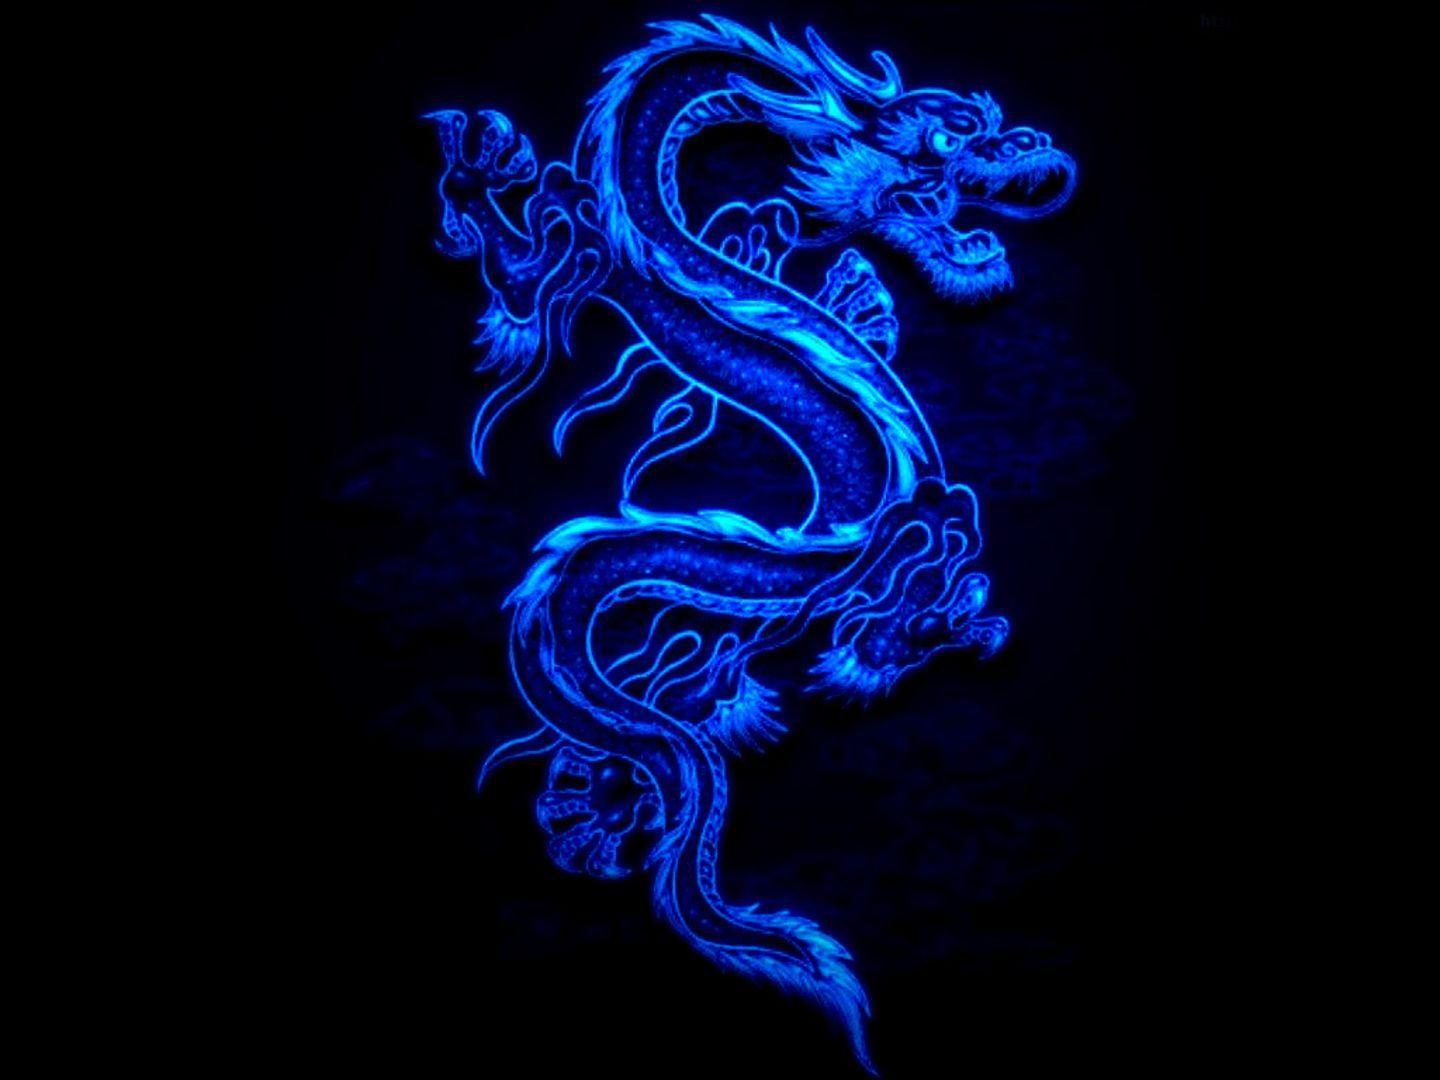
\includegraphics[width=0.5\textwidth,height=\textheight]{images/fun_dragon.jpg}

}

\caption{Dream pet dragon}

\end{figure}%

\part{Open Science}

\chapter{Introduction to open
Science}\label{introduction-to-open-science}

\section{Why do we need it?}\label{why-do-we-need-it}

\section{Lecture}\label{lecture}

\begin{figure}[H]

{\centering 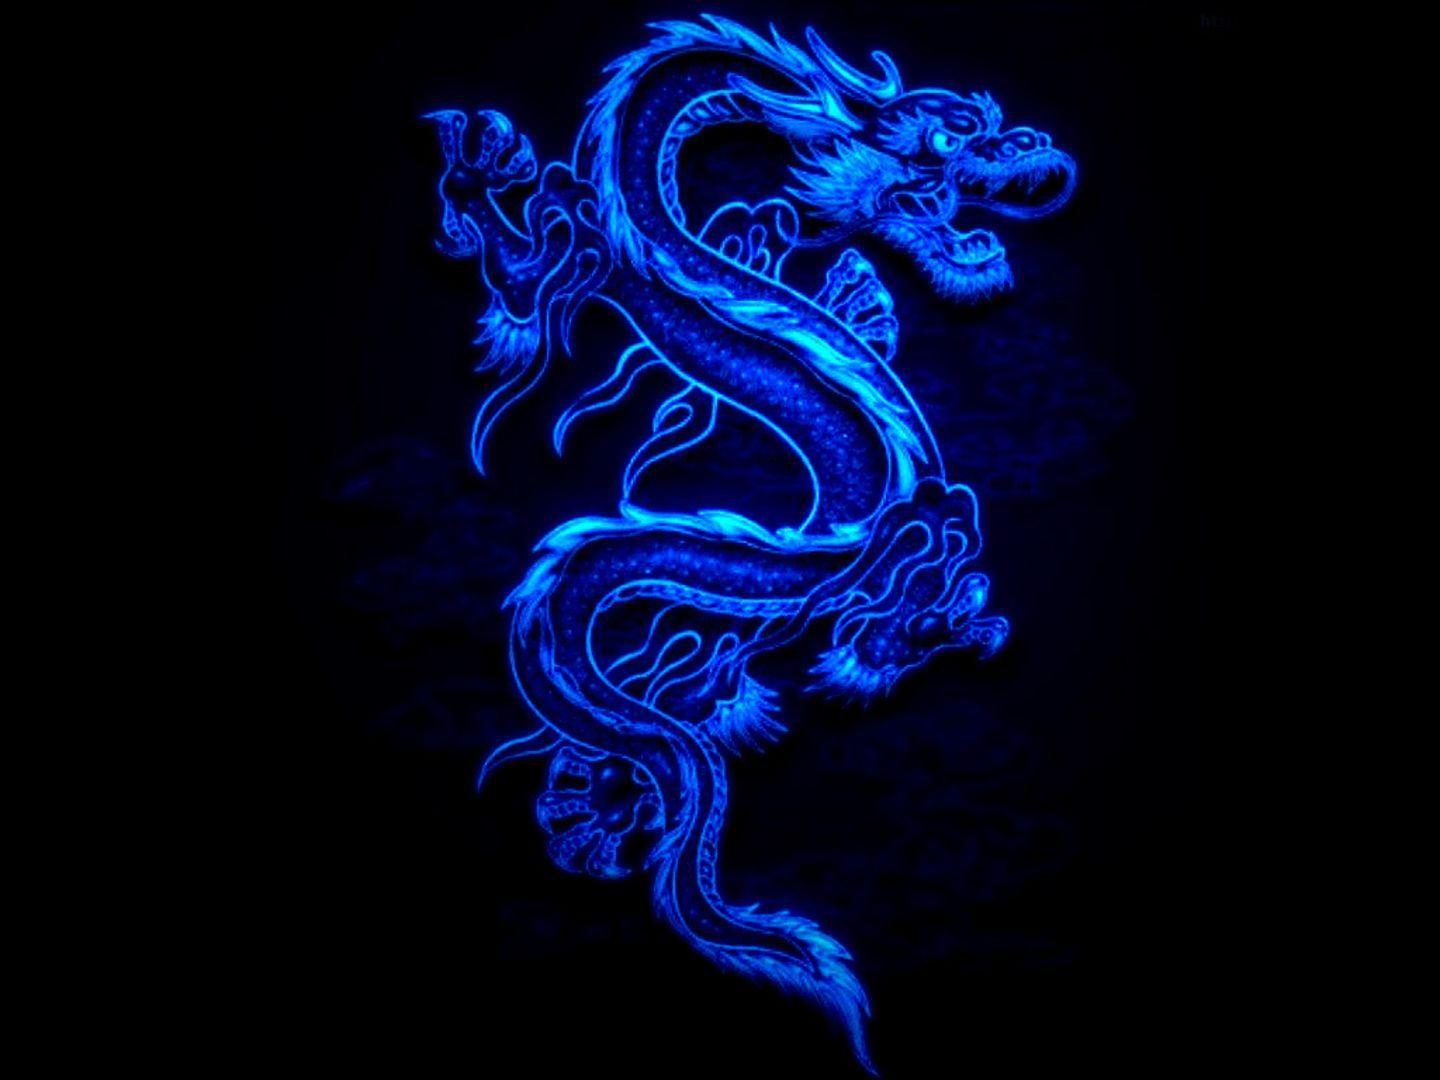
\includegraphics[width=0.5\textwidth,height=\textheight]{images/fun_dragon.jpg}

}

\caption{Dream pet dragon}

\end{figure}%

\section{What it is?}\label{what-it-is}

\section{Reproducible code and
analysis}\label{reproducible-code-and-analysis}

\chapter{Introduction to Rmarkdown}\label{introduction-to-rmarkdown}

\section{Lecture}\label{lecture-1}

\begin{figure}[H]

{\centering 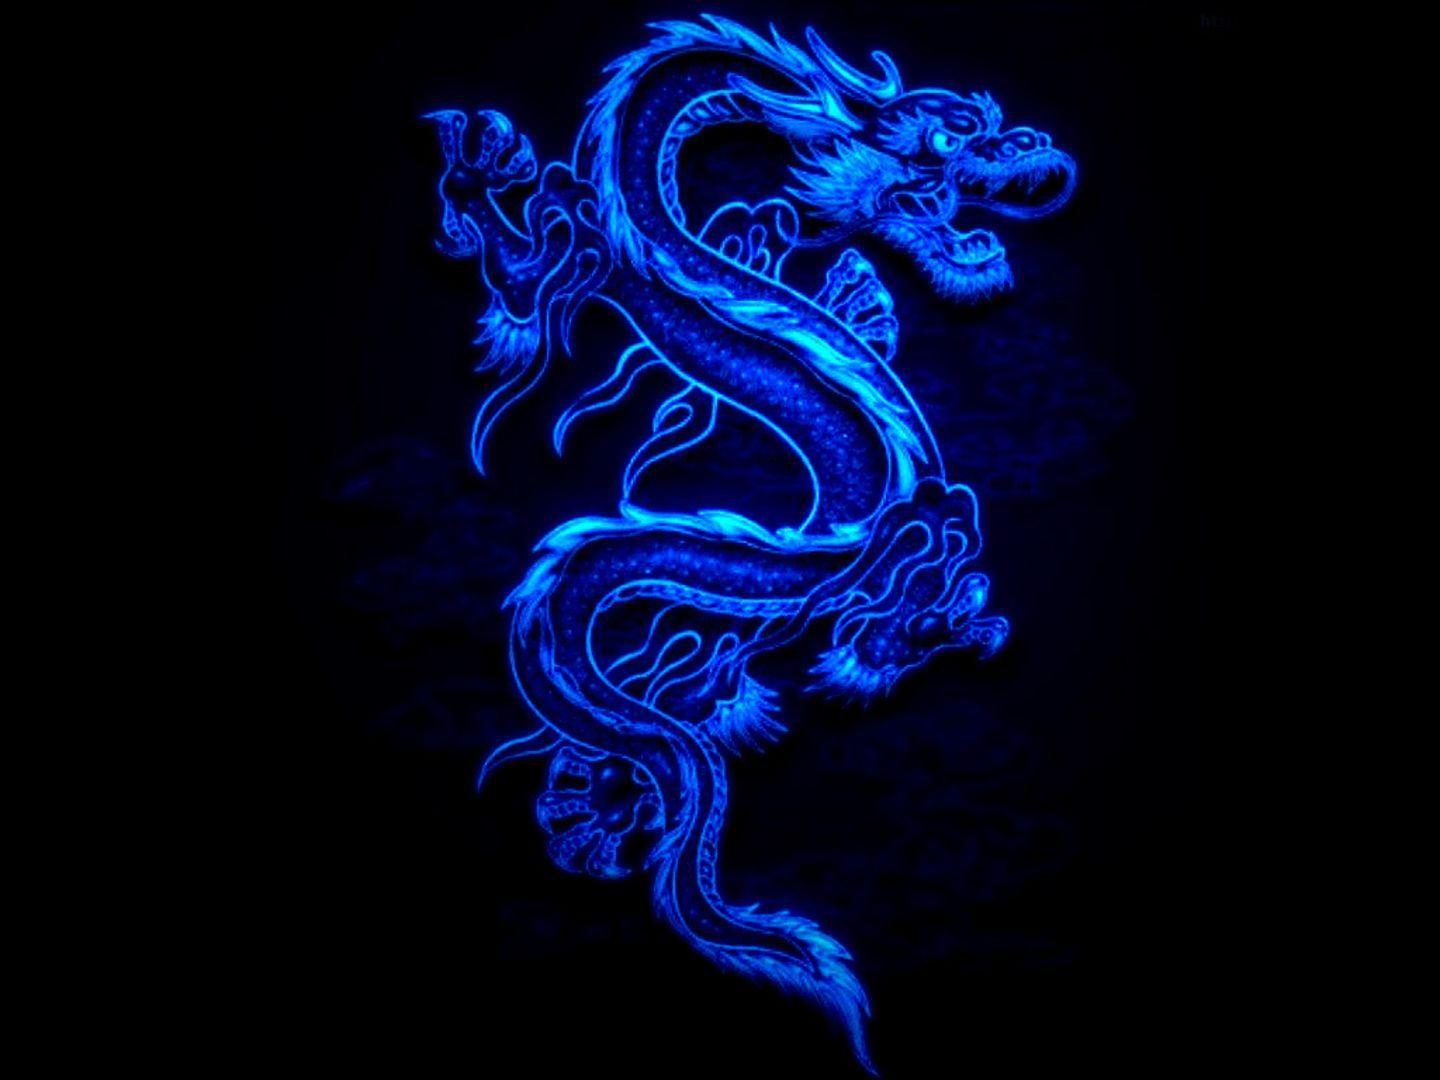
\includegraphics[width=0.5\textwidth,height=\textheight]{images/fun_dragon.jpg}

}

\caption{Dream pet dragon}

\end{figure}%

\section{Practical}\label{practical}

We will create a new Rmarkdown document and edit it using basic
\texttt{R} and \texttt{Rmarkdown} functions.

\subsection{Context}\label{context}

We will use the awesome \texttt{palmerpenguins} dataset 🐧 to explore
and visualize data.

These data have been collected and shared by
\href{https://www.uaf.edu/cfos/people/faculty/detail/kristen-gorman.php}{Dr.~Kristen
Gorman} and \href{https://pal.lternet.edu/}{Palmer Station, Antarctica
LTER}.

The package was built by Drs Allison Horst and Alison Hill, check out
the \href{https://allisonhorst.github.io/palmerpenguins/}{official
website}.

The package \texttt{palmerpenguins} has two datasets:

\begin{itemize}
\tightlist
\item
  \texttt{penguins\_raw} has the raw data of penguins observations (see
  \texttt{?penguins\_raw} for more info)
\item
  \texttt{penguins} is a simplified version of the raw data (see
  \texttt{?penguins} for more info)
\end{itemize}

For this exercise, we're gonna use the \texttt{penguins} dataset.

\begin{Shaded}
\begin{Highlighting}[]
\FunctionTok{library}\NormalTok{(palmerpenguins)}
\FunctionTok{head}\NormalTok{(penguins)}
\end{Highlighting}
\end{Shaded}

\begin{verbatim}
# A tibble: 6 x 8
  species island    bill_length_mm bill_depth_mm flipper_length_mm body_mass_g
  <fct>   <fct>              <dbl>         <dbl>             <int>       <int>
1 Adelie  Torgersen           39.1          18.7               181        3750
2 Adelie  Torgersen           39.5          17.4               186        3800
3 Adelie  Torgersen           40.3          18                 195        3250
4 Adelie  Torgersen           NA            NA                  NA          NA
5 Adelie  Torgersen           36.7          19.3               193        3450
6 Adelie  Torgersen           39.3          20.6               190        3650
# i 2 more variables: sex <fct>, year <int>
\end{verbatim}

\subsection{Questions}\label{questions}

\textbf{1)} Install the package \texttt{palmerpenguins}.

\begin{Shaded}
\begin{Highlighting}[]
\FunctionTok{install.packages}\NormalTok{(}\StringTok{"palmerpenguins"}\NormalTok{)}
\end{Highlighting}
\end{Shaded}

\textbf{2)}

\begin{itemize}
\tightlist
\item
  Create a new R Markdown document, name it and save it.
\item
  Delete everything after line 12.
\item
  Add a new section title, simple text and text in bold font.
\item
  Compile (``Knit'').
\end{itemize}

\textbf{3)}

\begin{itemize}
\tightlist
\item
  Add a chunk in which you load the \texttt{palmerpenguins}. The
  corresponding line of code should be hidden in the output.
\item
  Load also the \texttt{tidyverse} suite of packages. Modify the
  defaults to suppress all messages.
\end{itemize}

\begin{Shaded}
\begin{Highlighting}[]
\InformationTok{\textasciigrave{}\textasciigrave{}\textasciigrave{}\{r, echo = FALSE, message = FALSE\}}
\InformationTok{library(palmerpenguins)}
\InformationTok{library(tidyverse)}
\InformationTok{\textasciigrave{}\textasciigrave{}\textasciigrave{}}
\end{Highlighting}
\end{Shaded}

\textbf{4)} Add another chunk in which you build a table with the 10
first rows of the dataset.

\begin{Shaded}
\begin{Highlighting}[]
\InformationTok{\textasciigrave{}\textasciigrave{}\textasciigrave{}\{r\}}
\InformationTok{penguins \%\textgreater{}\%}
\InformationTok{  slice(1:10) \%\textgreater{}\%}
\InformationTok{  knitr::kable()}
\InformationTok{\textasciigrave{}\textasciigrave{}\textasciigrave{}}
\end{Highlighting}
\end{Shaded}

\textbf{5)} In a new section, display how many individuals, penguins
species and islands we have in the dataset. This info should appear
directly in the text, you need to use inline code 😄. Calculate the mean
of the (numeric) traits measured on the penguins.

\begin{Shaded}
\begin{Highlighting}[]
\FunctionTok{\#\# Numerical exploration}

\NormalTok{There are }\InformationTok{\textasciigrave{}r nrow(penguins)\textasciigrave{}}\NormalTok{ penguins in the dataset,}
\NormalTok{and }\InformationTok{\textasciigrave{}r length(unique(penguins$species))\textasciigrave{}}\NormalTok{ different species.}
\NormalTok{The data were collected in }\InformationTok{\textasciigrave{}r length(unique(penguins$island))\textasciigrave{}}
\NormalTok{islands of the Palmer archipelago in Antarctica.}

\NormalTok{The mean of all traits that were measured on the penguins are:}

\InformationTok{\textasciigrave{}\textasciigrave{}\textasciigrave{}\{r echo = FALSE\}}
\InformationTok{penguins \%\textgreater{}\%}
\InformationTok{  group\_by(species) \%\textgreater{}\%}
\InformationTok{  summarize(across(where(is.numeric), mean, na.rm = TRUE))}
\InformationTok{\textasciigrave{}\textasciigrave{}\textasciigrave{}}
\end{Highlighting}
\end{Shaded}

\textbf{6)} In another section, entitled `Graphical exploration', build
a figure with 3 superimposed histograms, each one corresponding to the
body mass of a species.

\begin{Shaded}
\begin{Highlighting}[]
\FunctionTok{\#\# Graphical exploration}

\NormalTok{A histogram of body mass per species:}

\InformationTok{\textasciigrave{}\textasciigrave{}\textasciigrave{}\{r, fig.cap = "Distribution of body mass by species of penguins"\}}
\InformationTok{  ggplot(data = penguins) +}
\InformationTok{  aes(x = body\_mass\_g) +}
\InformationTok{  geom\_histogram(aes(fill = species),}
\InformationTok{                 alpha = 0.5,}
\InformationTok{                 position = "identity") +}
\InformationTok{  scale\_fill\_manual(values = c("darkorange","purple","cyan4")) +}
\InformationTok{  theme\_minimal() +}
\InformationTok{  labs(x = "Body mass (g)",}
\InformationTok{       y = "Frequency",}
\InformationTok{       title = "Penguin body mass")}
\InformationTok{\textasciigrave{}\textasciigrave{}\textasciigrave{}}
\end{Highlighting}
\end{Shaded}

\textbf{7)} In another section, entitled \emph{Linear regression}, fit a
model of bill length as a function of body size (flipper length), body
mass and sex. Obtain the output and graphically evaluate the assumptions
of the model. As reminder here is how you fit a linear regression.

\begin{Shaded}
\begin{Highlighting}[]
\InformationTok{\textasciigrave{}\textasciigrave{}\textasciigrave{}\{r\}}
\InformationTok{model \textless{}{-} lm(Y \textasciitilde{}  X1 + X2, data = data)}
\InformationTok{summary(model)}
\InformationTok{plot(model)}
\InformationTok{\textasciigrave{}\textasciigrave{}\textasciigrave{}}
\end{Highlighting}
\end{Shaded}

\begin{Shaded}
\begin{Highlighting}[]
\FunctionTok{\#\# Linear regression}

\NormalTok{And here is a nice model with graphical output}

\InformationTok{\textasciigrave{}\textasciigrave{}\textasciigrave{}\{r, fig.cap = "Checking assumptions of the model"\}}
\InformationTok{m1 \textless{}{-} lm(bill\_length\_mm \textasciitilde{}  flipper\_length\_mm + body\_mass\_g + sex, data = penguins)}
\InformationTok{summary(m1)}
\InformationTok{par(mfrow= c(2,2))}
\InformationTok{plot(m1)}
\InformationTok{\textasciigrave{}\textasciigrave{}\textasciigrave{}}
\end{Highlighting}
\end{Shaded}

\textbf{8)} Add references manually or using \texttt{citr} in
\texttt{RStudio}.

\begin{enumerate}
\def\labelenumi{\arabic{enumi}.}
\tightlist
\item
  Pick a recent publication from the researcher who shared the data, Dr
  Kristen Gorman. Import this publication in your favorite references
  manager (we use Zotero, no hard feeling), and create a bibtex
  reference that you will add to to the file \texttt{mabiblio.bib}.
\item
  Add \texttt{bibliography:\ mabiblio.bib} at the beginning of your R
  Markdown document (YAML).
\item
  Cite the reference iin the text using either typing the reference
  manually or using \texttt{citr}. To use \texttt{citr}, instal it
  first; if everything goes well, you should see it in the pulldown menu
  \texttt{Addins} 💪. Then simply use \texttt{Insert\ citations} in the
  pull-down menu \texttt{Addins}.
\item
  Compile.
\end{enumerate}

\textbf{9)} Change the default citation format (Chicago style) into the
The American Naturalist format. It can be found here
\url{https://www.zotero.org/styles}. To do soo, add
\texttt{csl:\ the-american-naturalist.csl} in the YAML.

\textbf{10)} Build your report in html, pdf and docx format. 🎉

\subsection*{Example of output}\label{example-of-output}
\addcontentsline{toc}{subsection}{Example of output}

You can see an example of the
\href{data/examples/rmarkdown_practical.Rmd}{Rmarkdown source file} and
\href{data/examples/rmarkdown_practical.pdf}{pdf output}

\begin{figure}[H]

{\centering 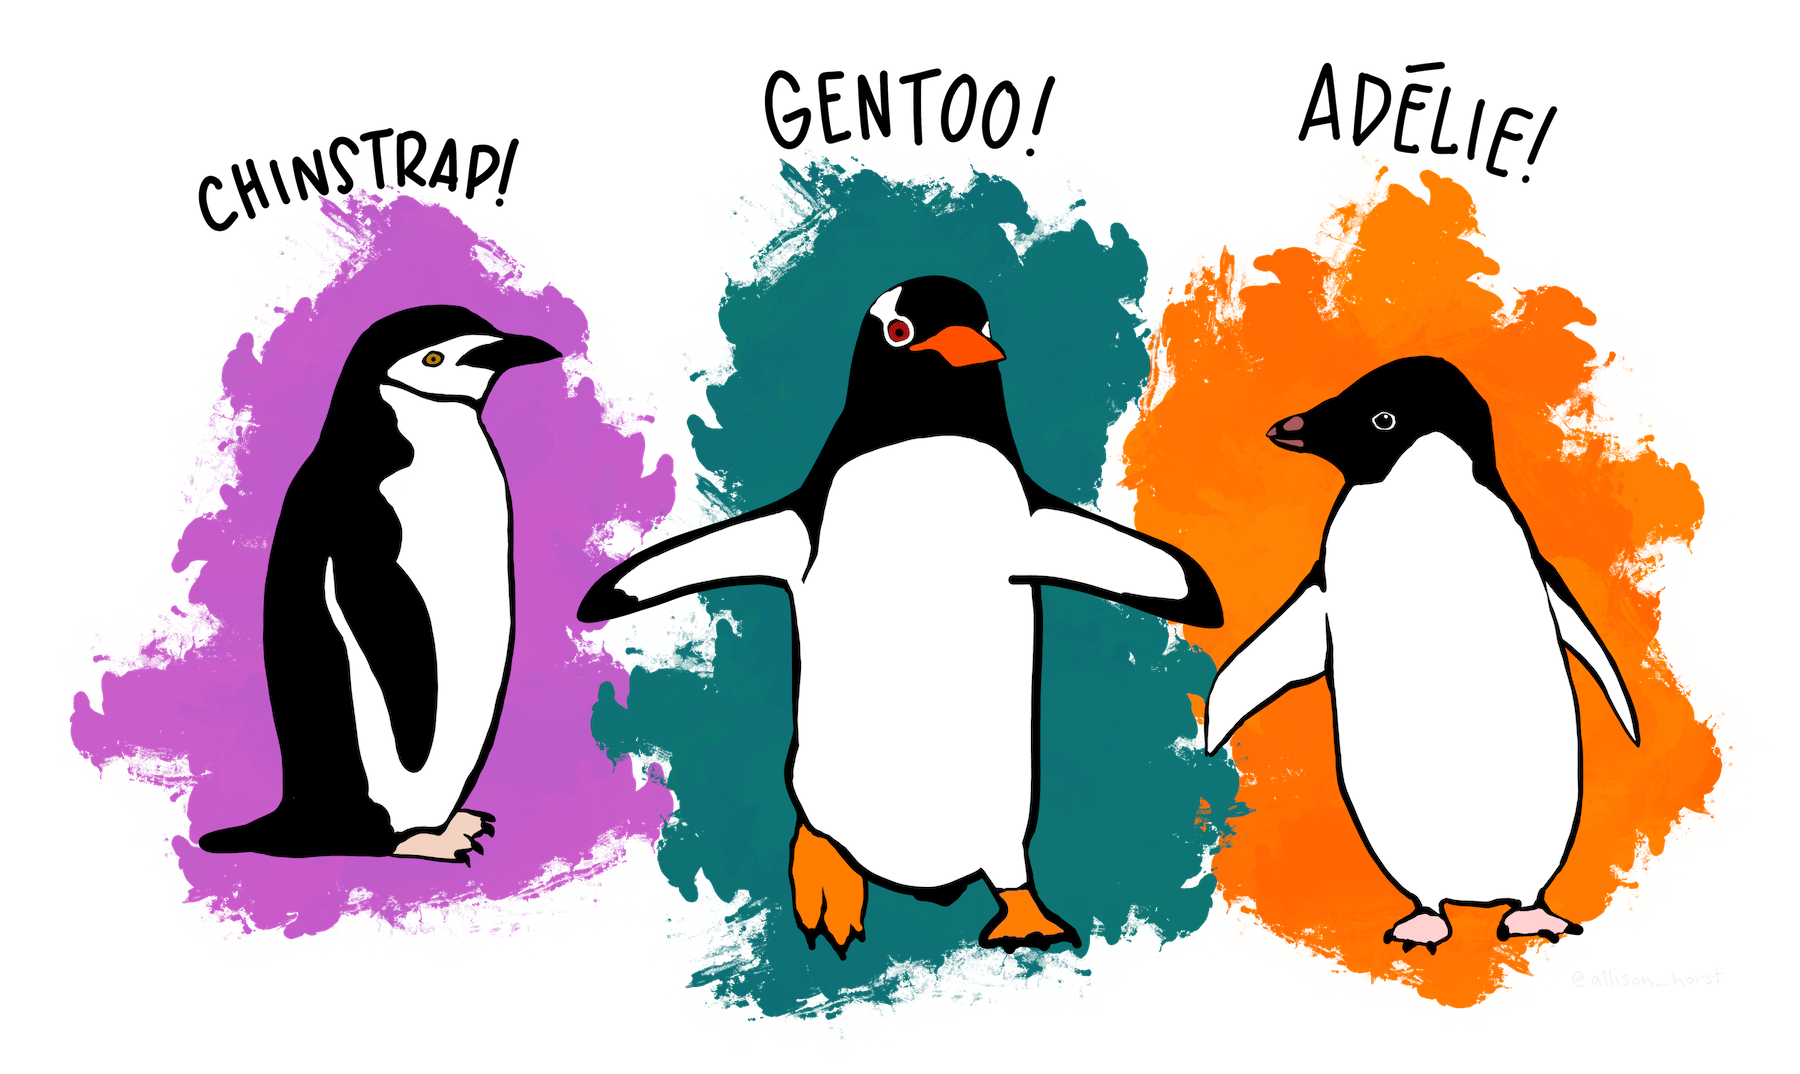
\includegraphics[width=0.5\textwidth,height=\textheight]{images/lter_penguins.png}

}

\caption{Happy coding}

\end{figure}%

\chapter{Introduction to github with
R}\label{introduction-to-github-with-r}

\section{Lecture}\label{lecture-2}

\begin{figure}[H]

{\centering 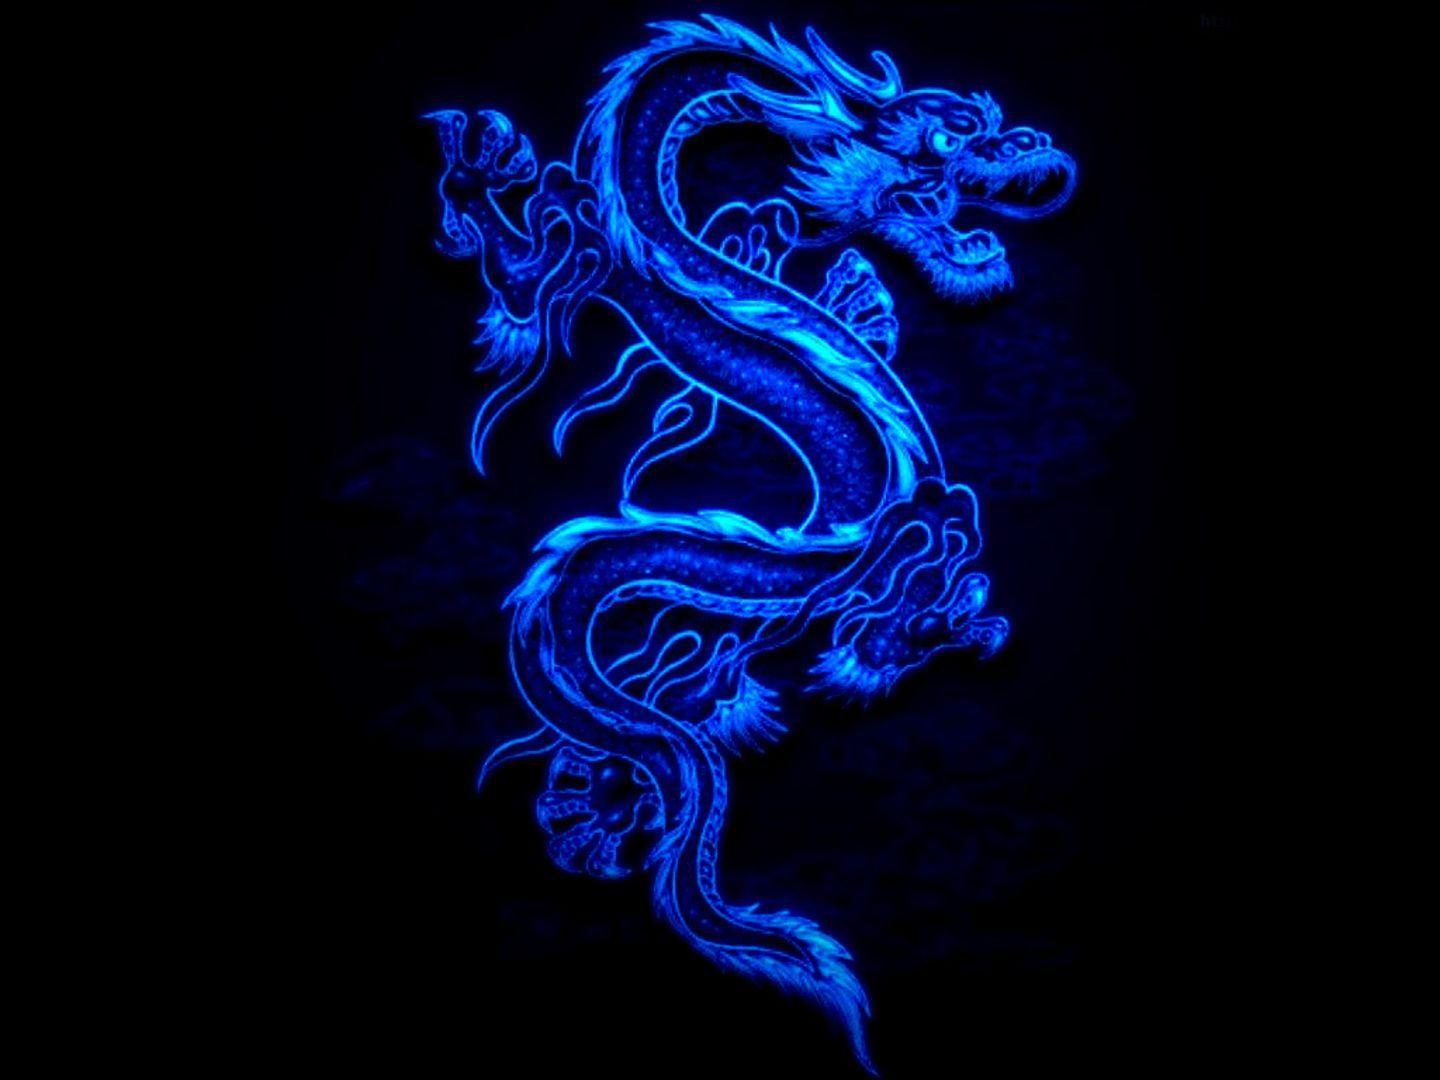
\includegraphics[width=0.5\textwidth,height=\textheight]{images/fun_dragon.jpg}

}

\caption{Dream pet dragon}

\end{figure}%

\section{Practical}\label{git_practical}

\subsection{Context}\label{context-1}

We will configure Rstudio to work with our github account, then create a
new project and start using \texttt{github}. To have some data I suggest
to use the awesome \texttt{palmerpenguins} dataset 🐧.

\subsection{Information of the data}\label{information-of-the-data}

These data have been collected and shared by
\href{https://www.uaf.edu/cfos/people/faculty/detail/kristen-gorman.php}{Dr.~Kristen
Gorman} and \href{https://pal.lternet.edu/}{Palmer Station, Antarctica
LTER}.

The package was built by Drs Allison Horst and Alison Hill, check out
the \href{https://allisonhorst.github.io/palmerpenguins/}{official
website}.

The package \texttt{palmerpenguins} has two datasets.

\begin{Shaded}
\begin{Highlighting}[]
\FunctionTok{library}\NormalTok{(palmerpenguins)}
\end{Highlighting}
\end{Shaded}

The dataset \texttt{penguins} is a simplified version of the raw data;
see \texttt{?penguins} for more info:

\begin{Shaded}
\begin{Highlighting}[]
\FunctionTok{head}\NormalTok{(penguins)}
\end{Highlighting}
\end{Shaded}

\begin{verbatim}
# A tibble: 6 x 8
  species island    bill_length_mm bill_depth_mm flipper_length_mm body_mass_g
  <fct>   <fct>              <dbl>         <dbl>             <int>       <int>
1 Adelie  Torgersen           39.1          18.7               181        3750
2 Adelie  Torgersen           39.5          17.4               186        3800
3 Adelie  Torgersen           40.3          18                 195        3250
4 Adelie  Torgersen           NA            NA                  NA          NA
5 Adelie  Torgersen           36.7          19.3               193        3450
6 Adelie  Torgersen           39.3          20.6               190        3650
# i 2 more variables: sex <fct>, year <int>
\end{verbatim}

The other dataset \texttt{penguins\_raw} has the raw data; see
\texttt{?penguins\_raw} for more info:

\begin{Shaded}
\begin{Highlighting}[]
\FunctionTok{head}\NormalTok{(penguins\_raw)}
\end{Highlighting}
\end{Shaded}

\begin{verbatim}
# A tibble: 6 x 17
  studyName `Sample Number` Species          Region Island Stage `Individual ID`
  <chr>               <dbl> <chr>            <chr>  <chr>  <chr> <chr>          
1 PAL0708                 1 Adelie Penguin ~ Anvers Torge~ Adul~ N1A1           
2 PAL0708                 2 Adelie Penguin ~ Anvers Torge~ Adul~ N1A2           
3 PAL0708                 3 Adelie Penguin ~ Anvers Torge~ Adul~ N2A1           
4 PAL0708                 4 Adelie Penguin ~ Anvers Torge~ Adul~ N2A2           
5 PAL0708                 5 Adelie Penguin ~ Anvers Torge~ Adul~ N3A1           
6 PAL0708                 6 Adelie Penguin ~ Anvers Torge~ Adul~ N3A2           
# i 10 more variables: `Clutch Completion` <chr>, `Date Egg` <date>,
#   `Culmen Length (mm)` <dbl>, `Culmen Depth (mm)` <dbl>,
#   `Flipper Length (mm)` <dbl>, `Body Mass (g)` <dbl>, Sex <chr>,
#   `Delta 15 N (o/oo)` <dbl>, `Delta 13 C (o/oo)` <dbl>, Comments <chr>
\end{verbatim}

For this exercise, we're gonna use the \texttt{penguins} dataset.

\subsection{Questions}\label{questions-1}

\textbf{1)} Create a github account if not done yet.

\textbf{2)} Configure Rstudio with your github account using the
\texttt{usethis} package.

\begin{Shaded}
\begin{Highlighting}[]
\NormalTok{usethis}\SpecialCharTok{::}\FunctionTok{git\_sitrep}\NormalTok{()}
\NormalTok{usethis}\SpecialCharTok{::}\FunctionTok{use\_git\_config}\NormalTok{(}
  \AttributeTok{user.name =} \StringTok{"your\_username"}\NormalTok{,}
  \AttributeTok{user.email =} \StringTok{"your\_email@address.com"}
\NormalTok{)}
\end{Highlighting}
\end{Shaded}

\textbf{3)} Create and Store your GITHUB Personal Authorisation Token

\begin{Shaded}
\begin{Highlighting}[]
\NormalTok{usethis}\SpecialCharTok{::}\FunctionTok{create\_github\_token}\NormalTok{()}
\NormalTok{gitcreds}\SpecialCharTok{::}\FunctionTok{gitcreds\_set}\NormalTok{()}
\end{Highlighting}
\end{Shaded}

\textbf{4)} Create a new R Markdown project, initialize it for git, and
create a new git repository

\begin{Shaded}
\begin{Highlighting}[]
\CommentTok{\#create R project}
\NormalTok{usethis}\SpecialCharTok{::}\FunctionTok{use\_git}\NormalTok{()}

\CommentTok{\#restart R}
\NormalTok{usethis}\SpecialCharTok{::}\FunctionTok{use\_github}\NormalTok{()}
\NormalTok{usethis}\SpecialCharTok{::}\FunctionTok{git\_vaccinate}\NormalTok{()}
\end{Highlighting}
\end{Shaded}

\textbf{5)} Create a new Rmarkdown document, in your project. Then save
the file and stage it.

\textbf{6)} Create a new commit including the new file and push it to
github (Check on github that it works).

\textbf{7)} Edit the file. Delete everything after line 12. Add a new
section title, simple text and text in bold font. Then knit and compile.

\textbf{8)} Make a new commit (with a meaningful message), and push to
github.

\textbf{9)} Create a new branch, and add a new section to the rmarkdown
file in this branch. Whatever you want. I would suggest a graph of the
data.

\textbf{10)} Create a commit and push it to the branch.

\textbf{11)} On github, create a pull request to merge the 2 different
branches.

\textbf{12)} Check and accept the pull request to merge the 2 branches.

You have successfully used all the essential tools of \texttt{git} 🎉 .
You are really to explore 🕵 and discover its power 💪

\begin{figure}[H]

{\centering 
\includegraphics[width=0.3\textwidth,height=\textheight]{images/github_ninja.jpg}

}

\caption{Happy git(hub)-ing}

\end{figure}%

\part{Statistics}

\chapter{\texorpdfstring{Generalized linear model,
\texttt{glm}}{Generalized linear model, glm}}\label{generalized-linear-model-glm}

\section{Lecture}\label{lecture-3}

\begin{figure}[H]

{\centering 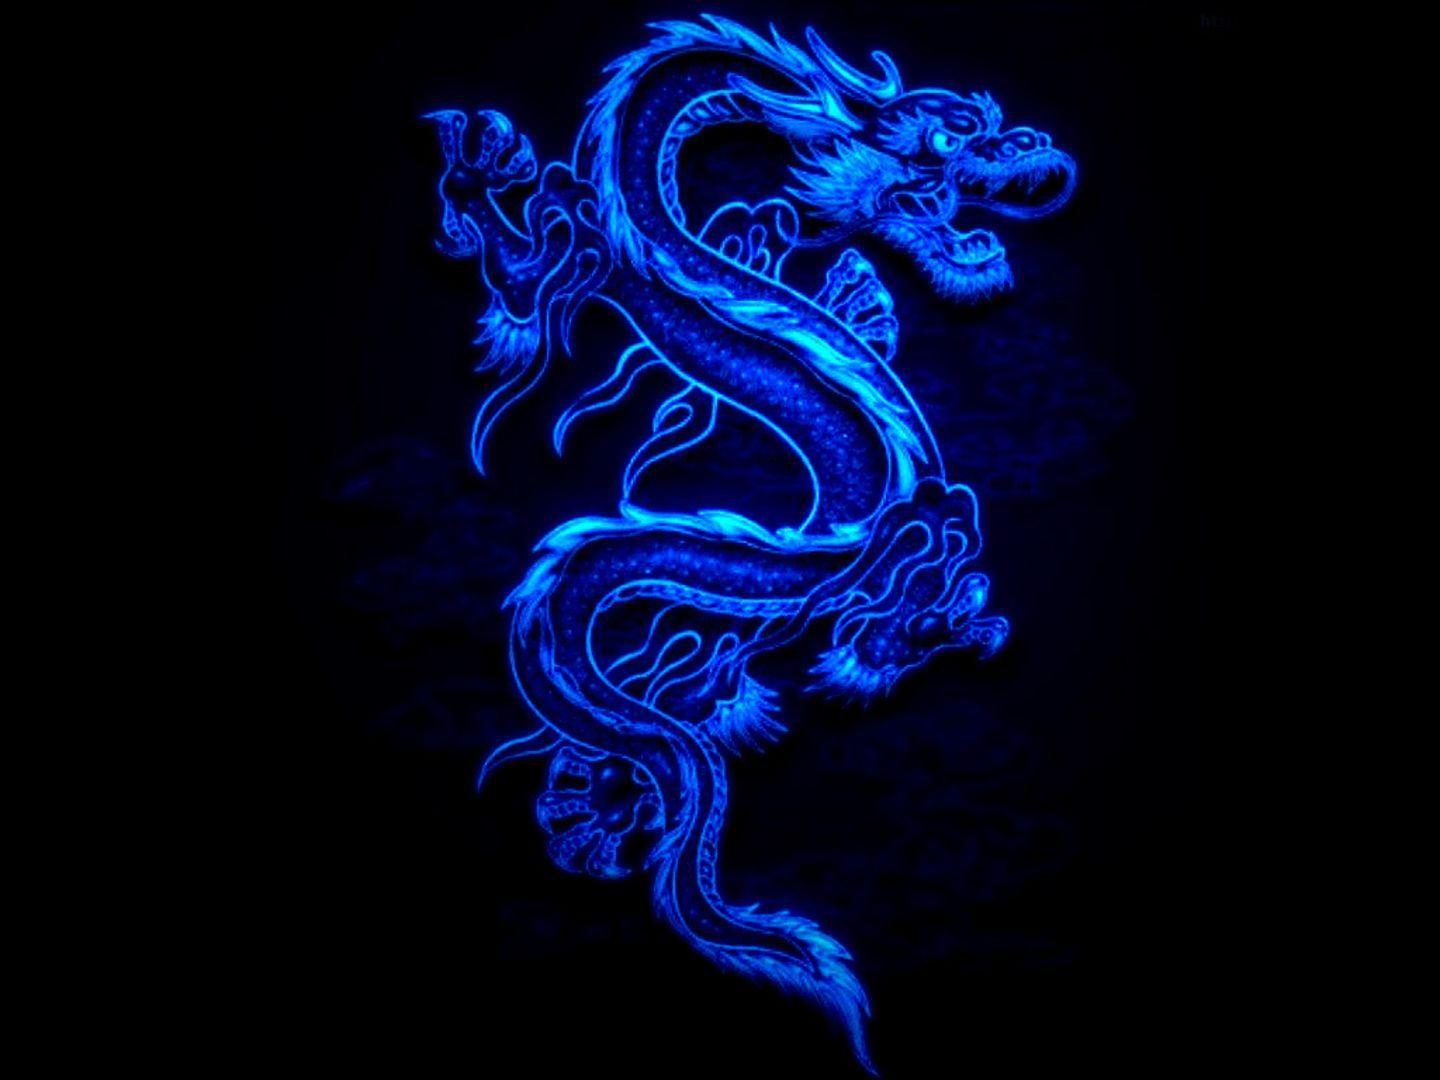
\includegraphics[width=0.5\textwidth,height=\textheight]{images/fun_dragon.jpg}

}

\caption{Dream pet dragon}

\end{figure}%

\begin{Shaded}
\begin{Highlighting}[]
\NormalTok{m1 }\OtherTok{\textless{}{-}} \FunctionTok{glm}\NormalTok{(fish }\SpecialCharTok{\textasciitilde{}}\NormalTok{ french\_captain, }\AttributeTok{data =}\NormalTok{ dads\_joke, }\AttributeTok{family =}\NormalTok{ poisson)}
\end{Highlighting}
\end{Shaded}

\subsection{Distributions}\label{distributions}

\subsubsection{Continuous linear}\label{continuous-linear}

\begin{itemize}
\tightlist
\item
  Gaussian
\end{itemize}

\subsubsection{Count data}\label{count-data}

\begin{itemize}
\tightlist
\item
  poisson
\item
  negative binomial
\item
  quasi-poisson
\item
  generalized poisson
\item
  conway-maxwell poisson
\end{itemize}

\subsubsection{censored distribution}\label{censored-distribution}

\subsubsection{zero-inflated / hurdle
distribution}\label{zero-inflated-hurdle-distribution}

\begin{itemize}
\tightlist
\item
  zero-inflated/zero-truncated poisson
\item
  censored poisson
\end{itemize}

\subsubsection{zero-truncated
distribution}\label{zero-truncated-distribution}

\subsubsection{zero-one-inflated
distribution}\label{zero-one-inflated-distribution}

see
https://cran.r-project.org/web/packages/brms/vignettes/brms\_families.html
see alo MCMCglmm coursenotes

for help on description and to add some plots about those distribution

\section{Practical}\label{practical-1}

::: \{.infobox .warning data-latex=``warning''\} This section need to
be severely updated :::

\subsection{Logistic regression}\label{logistic-regression}

\begin{Shaded}
\begin{Highlighting}[]
\FunctionTok{library}\NormalTok{(tidyverse)}
\end{Highlighting}
\end{Shaded}

\begin{verbatim}
-- Attaching core tidyverse packages ------------------------ tidyverse 2.0.0 --
v dplyr     1.1.4     v readr     2.1.5
v forcats   1.0.0     v stringr   1.5.1
v ggplot2   3.4.4     v tibble    3.2.1
v lubridate 1.9.3     v tidyr     1.3.0
v purrr     1.0.2     
-- Conflicts ------------------------------------------ tidyverse_conflicts() --
x dplyr::filter() masks stats::filter()
x dplyr::lag()    masks stats::lag()
i Use the conflicted package (<http://conflicted.r-lib.org/>) to force all conflicts to become errors
\end{verbatim}

\begin{Shaded}
\begin{Highlighting}[]
\FunctionTok{library}\NormalTok{(DHARMa)}
\end{Highlighting}
\end{Shaded}

\begin{verbatim}
This is DHARMa 0.4.6. For overview type '?DHARMa'. For recent changes, type news(package = 'DHARMa')
\end{verbatim}

\begin{Shaded}
\begin{Highlighting}[]
\FunctionTok{library}\NormalTok{(performance)}

\NormalTok{mouflon }\OtherTok{\textless{}{-}} \FunctionTok{read.csv}\NormalTok{(}\StringTok{"data/mouflon.csv"}\NormalTok{)}
\NormalTok{mouflonc }\OtherTok{\textless{}{-}}\NormalTok{ mouflon[}\FunctionTok{order}\NormalTok{(mouflon}\SpecialCharTok{$}\NormalTok{age),]}

\NormalTok{mouflonc}\SpecialCharTok{$}\NormalTok{reproduction }\OtherTok{\textless{}{-}} \FunctionTok{ifelse}\NormalTok{(mouflonc}\SpecialCharTok{$}\NormalTok{age }\SpecialCharTok{\textless{}} \DecValTok{13}\NormalTok{, mouflonc}\SpecialCharTok{$}\NormalTok{reproduction, }\DecValTok{0}\NormalTok{)}
\NormalTok{mouflonc}\SpecialCharTok{$}\NormalTok{reproduction }\OtherTok{\textless{}{-}} \FunctionTok{ifelse}\NormalTok{(mouflonc}\SpecialCharTok{$}\NormalTok{age }\SpecialCharTok{\textgreater{}} \DecValTok{4}\NormalTok{, mouflonc}\SpecialCharTok{$}\NormalTok{reproduction, }\DecValTok{1}\NormalTok{)}

\FunctionTok{plot}\NormalTok{(reproduction }\SpecialCharTok{\textasciitilde{}}\NormalTok{ age, mouflonc)}
\end{Highlighting}
\end{Shaded}

\includegraphics{02_01-glm_files/figure-pdf/unnamed-chunk-3-1.pdf}

\begin{Shaded}
\begin{Highlighting}[]
\FunctionTok{plot}\NormalTok{(}\FunctionTok{jitter}\NormalTok{(reproduction) }\SpecialCharTok{\textasciitilde{}} \FunctionTok{jitter}\NormalTok{(age), mouflonc)}
\end{Highlighting}
\end{Shaded}

\includegraphics{02_01-glm_files/figure-pdf/unnamed-chunk-3-2.pdf}

\begin{Shaded}
\begin{Highlighting}[]
\NormalTok{bubble }\OtherTok{\textless{}{-}} \FunctionTok{data.frame}\NormalTok{(}\AttributeTok{age =} \FunctionTok{rep}\NormalTok{(}\DecValTok{2}\SpecialCharTok{:}\DecValTok{16}\NormalTok{, }\DecValTok{2}\NormalTok{),}
                     \AttributeTok{reproduction =} \FunctionTok{rep}\NormalTok{(}\DecValTok{0}\SpecialCharTok{:}\DecValTok{1}\NormalTok{, }\AttributeTok{each =} \DecValTok{15}\NormalTok{),}
                     \AttributeTok{size =} \FunctionTok{c}\NormalTok{(}\FunctionTok{table}\NormalTok{(mouflonc}\SpecialCharTok{$}\NormalTok{age, mouflonc}\SpecialCharTok{$}\NormalTok{reproduction)))}
\NormalTok{bubble}\SpecialCharTok{$}\NormalTok{size }\OtherTok{\textless{}{-}} \FunctionTok{ifelse}\NormalTok{(bubble}\SpecialCharTok{$}\NormalTok{size }\SpecialCharTok{==} \DecValTok{0}\NormalTok{ , }\ConstantTok{NA}\NormalTok{, bubble}\SpecialCharTok{$}\NormalTok{size)}
 \FunctionTok{ggplot}\NormalTok{(}\AttributeTok{data =}\NormalTok{ bubble, }\FunctionTok{aes}\NormalTok{(}\AttributeTok{x =}\NormalTok{ age, }\AttributeTok{y =}\NormalTok{ reproduction))}\SpecialCharTok{+}
 \FunctionTok{geom\_point}\NormalTok{(}\FunctionTok{aes}\NormalTok{(}\AttributeTok{size =}\NormalTok{ size}\SpecialCharTok{*}\DecValTok{10}\NormalTok{))}
\end{Highlighting}
\end{Shaded}

\begin{verbatim}
Warning: Removed 7 rows containing missing values (`geom_point()`).
\end{verbatim}

\includegraphics{02_01-glm_files/figure-pdf/unnamed-chunk-3-3.pdf}

\begin{Shaded}
\begin{Highlighting}[]
\NormalTok{m1 }\OtherTok{\textless{}{-}} \FunctionTok{glm}\NormalTok{(reproduction }\SpecialCharTok{\textasciitilde{}}\NormalTok{ age,}
    \AttributeTok{data =}\NormalTok{ mouflonc,}
    \AttributeTok{family =}\NormalTok{ binomial)}
\FunctionTok{summary}\NormalTok{(m1)}
\end{Highlighting}
\end{Shaded}

\begin{verbatim}

Call:
glm(formula = reproduction ~ age, family = binomial, data = mouflonc)

Coefficients:
            Estimate Std. Error z value Pr(>|z|)    
(Intercept)  3.19921    0.25417   12.59   <2e-16 ***
age         -0.36685    0.03287  -11.16   <2e-16 ***
---
Signif. codes:  0 '***' 0.001 '**' 0.01 '*' 0.05 '.' 0.1 ' ' 1

(Dispersion parameter for binomial family taken to be 1)

    Null deviance: 928.86  on 715  degrees of freedom
Residual deviance: 767.51  on 714  degrees of freedom
  (4 observations deleted due to missingness)
AIC: 771.51

Number of Fisher Scoring iterations: 4
\end{verbatim}

\begin{Shaded}
\begin{Highlighting}[]
\NormalTok{simulationOutput }\OtherTok{\textless{}{-}} \FunctionTok{simulateResiduals}\NormalTok{(m1)}
\FunctionTok{plot}\NormalTok{(simulationOutput)}
\end{Highlighting}
\end{Shaded}

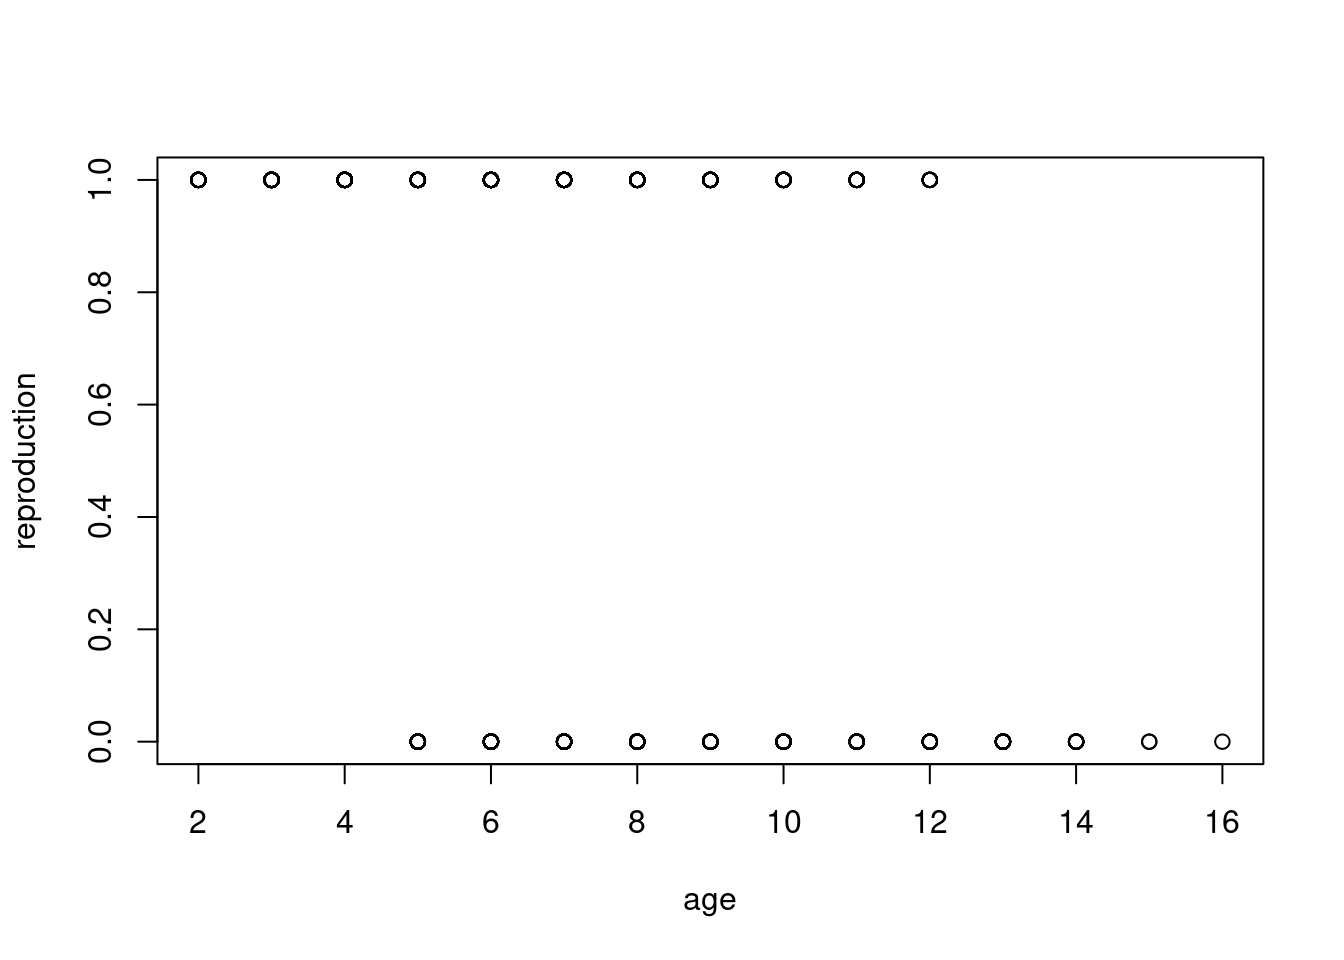
\includegraphics{02_01-glm_files/figure-pdf/unnamed-chunk-4-1.pdf}

plotting the model prediction on the link (latent) scale

\begin{Shaded}
\begin{Highlighting}[]
\NormalTok{mouflonc}\SpecialCharTok{$}\NormalTok{logit\_ypred }\OtherTok{\textless{}{-}} \FloatTok{3.19921} \SpecialCharTok{{-}}\FloatTok{0.36685} \SpecialCharTok{*}\NormalTok{ mouflonc}\SpecialCharTok{$}\NormalTok{age}
\FunctionTok{plot}\NormalTok{(logit\_ypred }\SpecialCharTok{\textasciitilde{}}  \FunctionTok{jitter}\NormalTok{(age), mouflonc)}
\FunctionTok{points}\NormalTok{(mouflonc}\SpecialCharTok{$}\NormalTok{age, mouflonc}\SpecialCharTok{$}\NormalTok{logit\_ypred, }\AttributeTok{col=}\StringTok{"red"}\NormalTok{, }\AttributeTok{type =} \StringTok{"l"}\NormalTok{, }\AttributeTok{lwd =} \DecValTok{2}\NormalTok{)}
\end{Highlighting}
\end{Shaded}

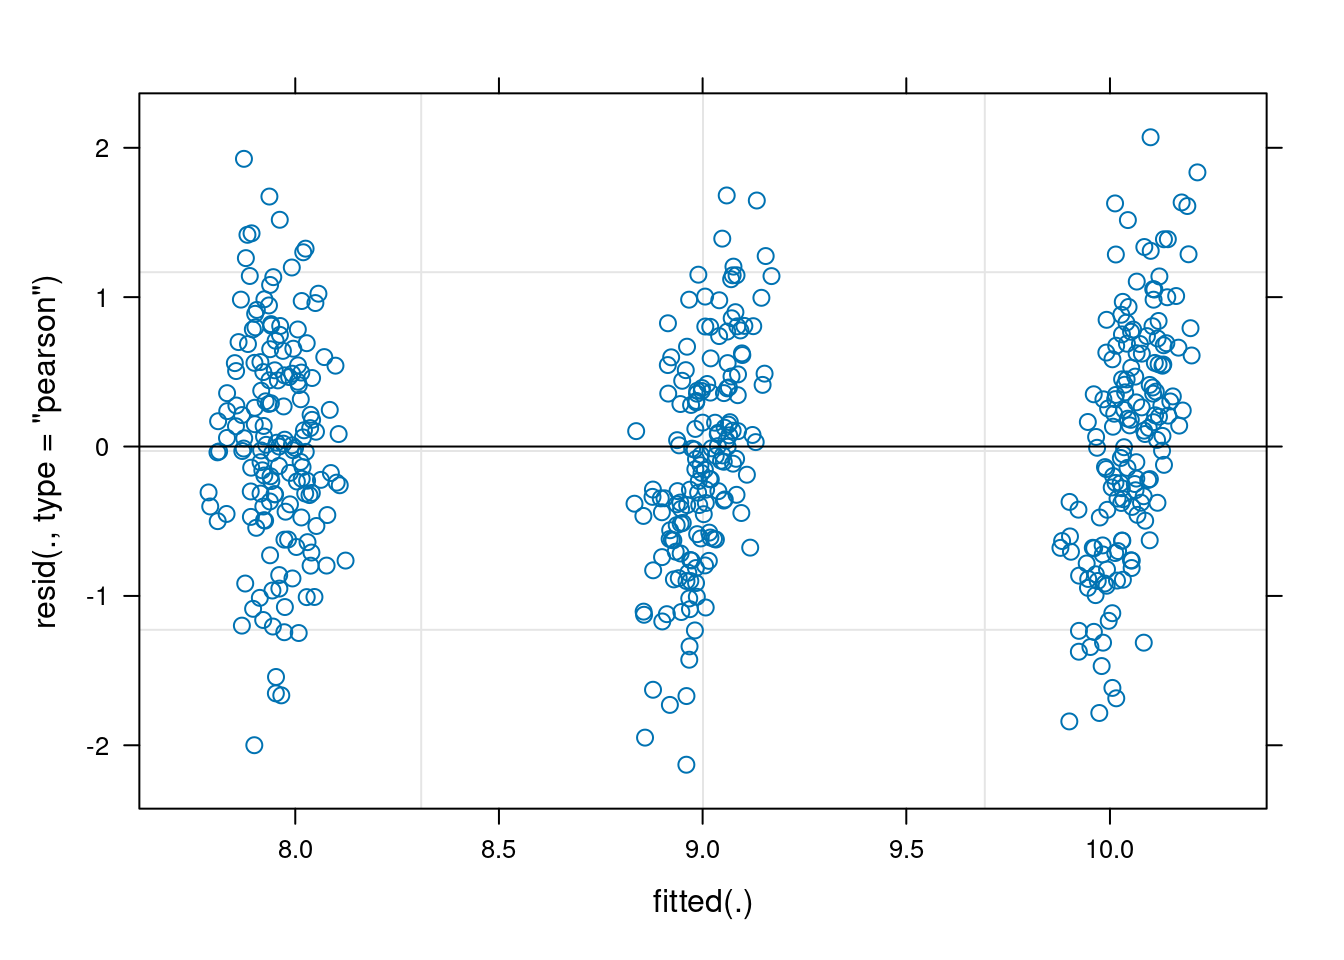
\includegraphics{02_01-glm_files/figure-pdf/unnamed-chunk-5-1.pdf}

plotting on the observed scale

\begin{Shaded}
\begin{Highlighting}[]
\NormalTok{mouflonc}\SpecialCharTok{$}\NormalTok{ypred }\OtherTok{\textless{}{-}} \FunctionTok{exp}\NormalTok{(mouflonc}\SpecialCharTok{$}\NormalTok{logit\_ypred) }\SpecialCharTok{/}\NormalTok{ (}\DecValTok{1} \SpecialCharTok{+} \FunctionTok{exp}\NormalTok{(mouflonc}\SpecialCharTok{$}\NormalTok{logit\_ypred)) }\CommentTok{\# inverse of logit }

\FunctionTok{plot}\NormalTok{(reproduction }\SpecialCharTok{\textasciitilde{}}  \FunctionTok{jitter}\NormalTok{(age), mouflonc)}
\FunctionTok{points}\NormalTok{(mouflonc}\SpecialCharTok{$}\NormalTok{age, mouflonc}\SpecialCharTok{$}\NormalTok{ypred, }\AttributeTok{col=}\StringTok{"red"}\NormalTok{, }\AttributeTok{type =} \StringTok{"l"}\NormalTok{, }\AttributeTok{lwd =} \DecValTok{2}\NormalTok{)}
\end{Highlighting}
\end{Shaded}

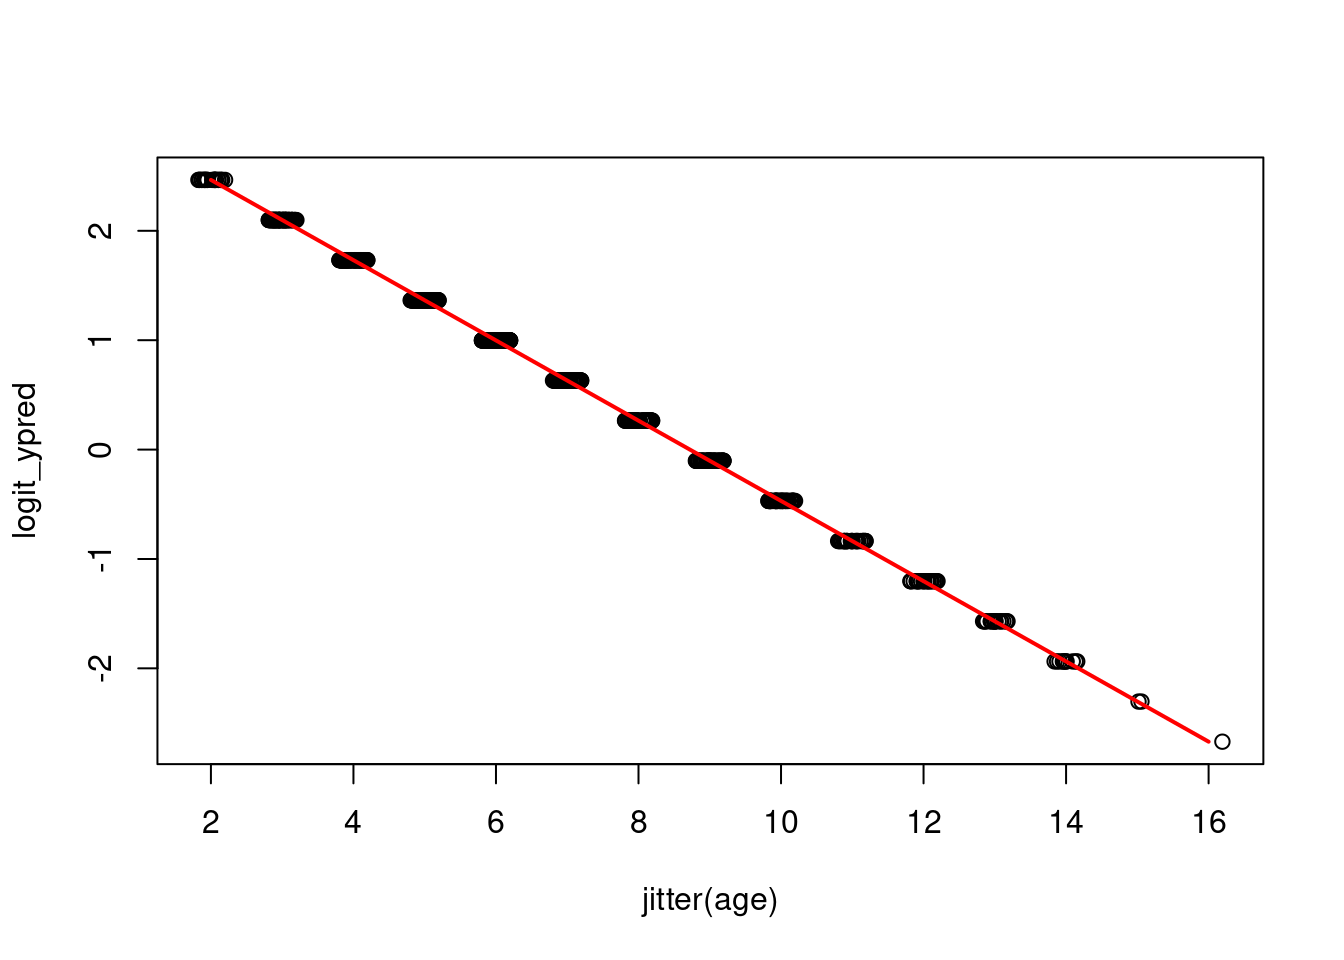
\includegraphics{02_01-glm_files/figure-pdf/unnamed-chunk-6-1.pdf}

Enfin, pour se simplifier la vie, il est aussi possible de récupérer les
valeurs prédites de y directement

\begin{Shaded}
\begin{Highlighting}[]
\FunctionTok{plot}\NormalTok{(x,y)}
\NormalTok{myreg }\OtherTok{\textless{}{-}} \FunctionTok{glm}\NormalTok{(y}\SpecialCharTok{\textasciitilde{}}\NormalTok{x, }\AttributeTok{family=}\FunctionTok{binomial}\NormalTok{(}\AttributeTok{link=}\NormalTok{logit))}
\NormalTok{ypredit }\OtherTok{\textless{}{-}}\NormalTok{ myreg}\SpecialCharTok{$}\NormalTok{fitted}
\NormalTok{o}\OtherTok{=}\FunctionTok{order}\NormalTok{(x)}
\FunctionTok{points}\NormalTok{(x[o],ypredit[o], }\AttributeTok{col=}\StringTok{"red"}\NormalTok{, }\AttributeTok{type=}\StringTok{"l"}\NormalTok{, }\AttributeTok{lwd=}\DecValTok{2}\NormalTok{)}
\end{Highlighting}
\end{Shaded}

\begin{Shaded}
\begin{Highlighting}[]
\NormalTok{m2 }\OtherTok{\textless{}{-}} \FunctionTok{glm}\NormalTok{(reproduction }\SpecialCharTok{\textasciitilde{}}\NormalTok{ age }\SpecialCharTok{+}\NormalTok{ mass\_sept }\SpecialCharTok{+} \FunctionTok{as.factor}\NormalTok{(sex\_lamb) }\SpecialCharTok{+}\NormalTok{ mass\_gain }\SpecialCharTok{+}\NormalTok{ density }\SpecialCharTok{+}\NormalTok{ temp,}
    \AttributeTok{data =}\NormalTok{ mouflon,}
    \AttributeTok{family =}\NormalTok{ binomial)}

\FunctionTok{summary}\NormalTok{(m2)}
\end{Highlighting}
\end{Shaded}

\begin{verbatim}

Call:
glm(formula = reproduction ~ age + mass_sept + as.factor(sex_lamb) + 
    mass_gain + density + temp, family = binomial, data = mouflon)

Coefficients:
                      Estimate Std. Error z value Pr(>|z|)    
(Intercept)           1.622007   1.943242   0.835 0.403892    
age                  -0.148567   0.033597  -4.422 9.78e-06 ***
mass_sept             0.029878   0.016815   1.777 0.075590 .  
as.factor(sex_lamb)1 -0.428169   0.166156  -2.577 0.009969 ** 
mass_gain            -0.094828   0.026516  -3.576 0.000348 ***
density              -0.018132   0.003518  -5.154 2.55e-07 ***
temp                  0.037244   0.138712   0.269 0.788313    
---
Signif. codes:  0 '***' 0.001 '**' 0.01 '*' 0.05 '.' 0.1 ' ' 1

(Dispersion parameter for binomial family taken to be 1)

    Null deviance: 916.06  on 674  degrees of freedom
Residual deviance: 845.82  on 668  degrees of freedom
  (45 observations deleted due to missingness)
AIC: 859.82

Number of Fisher Scoring iterations: 4
\end{verbatim}

\begin{Shaded}
\begin{Highlighting}[]
\FunctionTok{check\_model}\NormalTok{(m2)}
\end{Highlighting}
\end{Shaded}

\includegraphics{02_01-glm_files/figure-pdf/unnamed-chunk-8-1.pdf}

\begin{Shaded}
\begin{Highlighting}[]
\NormalTok{simulationOutput }\OtherTok{\textless{}{-}} \FunctionTok{simulateResiduals}\NormalTok{(m2)}
\FunctionTok{plot}\NormalTok{(simulationOutput)}
\end{Highlighting}
\end{Shaded}

\includegraphics{02_01-glm_files/figure-pdf/unnamed-chunk-8-2.pdf}

\subsubsection{previous offspring sex
effect}\label{previous-offspring-sex-effect}

\begin{Shaded}
\begin{Highlighting}[]
\NormalTok{pred.data }\OtherTok{\textless{}{-}} \FunctionTok{data.frame}\NormalTok{(}
  \AttributeTok{age =} \FunctionTok{mean}\NormalTok{(mouflon}\SpecialCharTok{$}\NormalTok{age),}
  \AttributeTok{mass\_sept =} \FunctionTok{mean}\NormalTok{(mouflon}\SpecialCharTok{$}\NormalTok{mass\_sept),}
  \AttributeTok{sex\_lamb =} \FunctionTok{c}\NormalTok{(}\DecValTok{0}\NormalTok{,}\DecValTok{1}\NormalTok{),}
  \AttributeTok{mass\_gain =} \FunctionTok{mean}\NormalTok{(mouflon}\SpecialCharTok{$}\NormalTok{mass\_gain),}
  \AttributeTok{density =} \FunctionTok{mean}\NormalTok{(mouflon}\SpecialCharTok{$}\NormalTok{density),}
  \AttributeTok{temp =} \FunctionTok{mean}\NormalTok{(mouflon}\SpecialCharTok{$}\NormalTok{temp, }\AttributeTok{na.rm =}\ConstantTok{TRUE}\NormalTok{))}

  \FunctionTok{predict}\NormalTok{(m2, }\AttributeTok{newdata =}\NormalTok{ pred.data)}
\end{Highlighting}
\end{Shaded}

\begin{verbatim}
        1         2 
0.6225895 0.1944205 
\end{verbatim}

\subsection{Poisson regression}\label{poisson-regression}

data on galapagos islands species richness model of total number of
species model of proportion of native model of density of species

Fit 3 models - model of total number of species - model of proportion of
endemics to total - model of species density

\begin{Shaded}
\begin{Highlighting}[]
  \FunctionTok{hist}\NormalTok{(}\FunctionTok{rpois}\NormalTok{(}\DecValTok{10000}\NormalTok{,}\DecValTok{3}\NormalTok{))}
\end{Highlighting}
\end{Shaded}

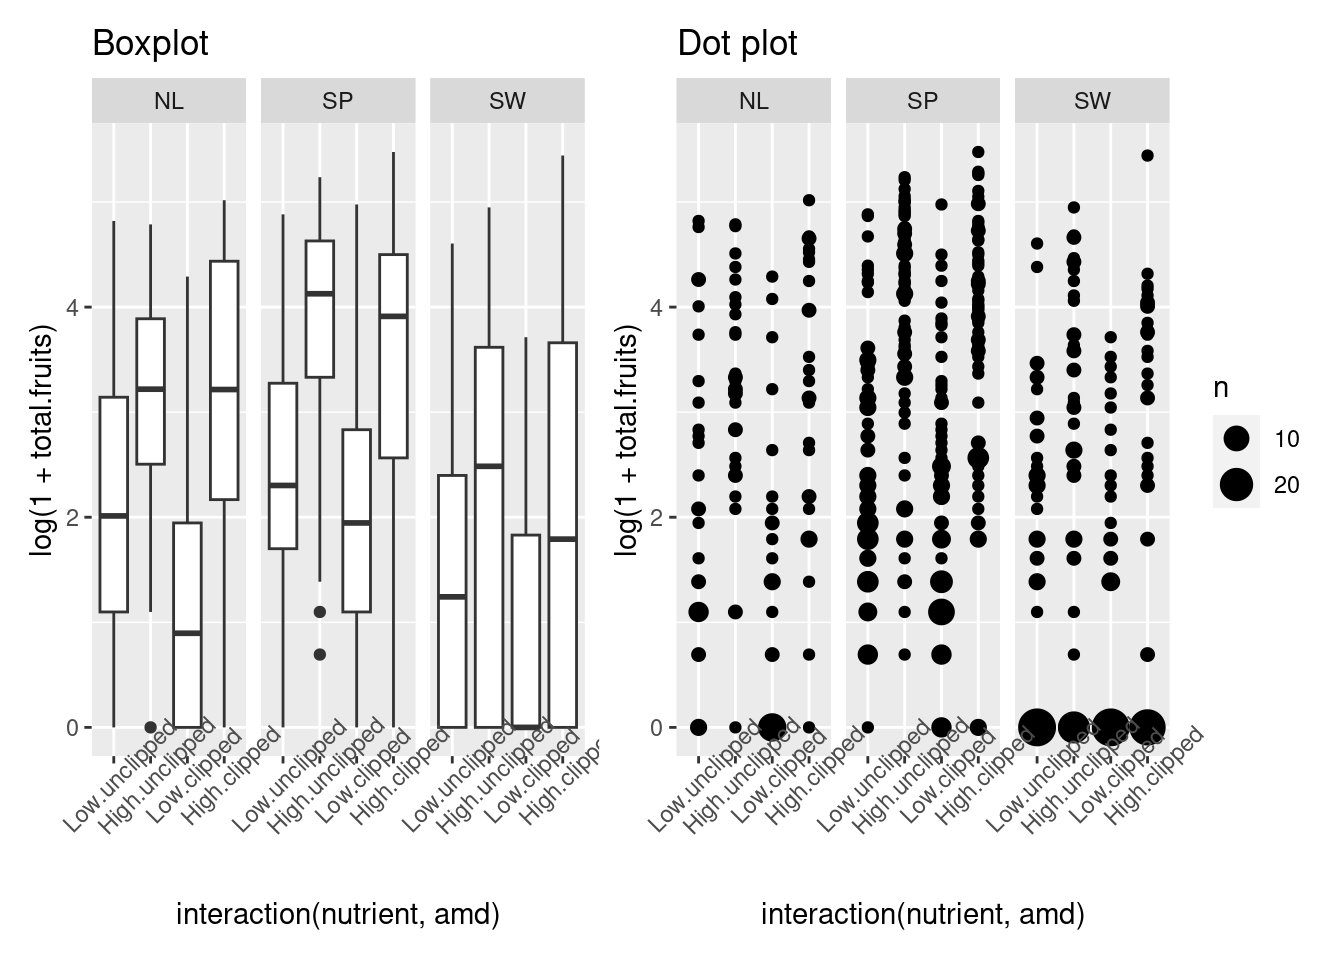
\includegraphics{02_01-glm_files/figure-pdf/unnamed-chunk-10-1.pdf}

\begin{Shaded}
\begin{Highlighting}[]
\CommentTok{\#}
\NormalTok{ gala }\OtherTok{\textless{}{-}} \FunctionTok{read.delim2}\NormalTok{(}\StringTok{"data/gala.txt"}\NormalTok{)}
 \FunctionTok{plot}\NormalTok{(Species }\SpecialCharTok{\textasciitilde{}}\NormalTok{ Area, gala)}
\end{Highlighting}
\end{Shaded}

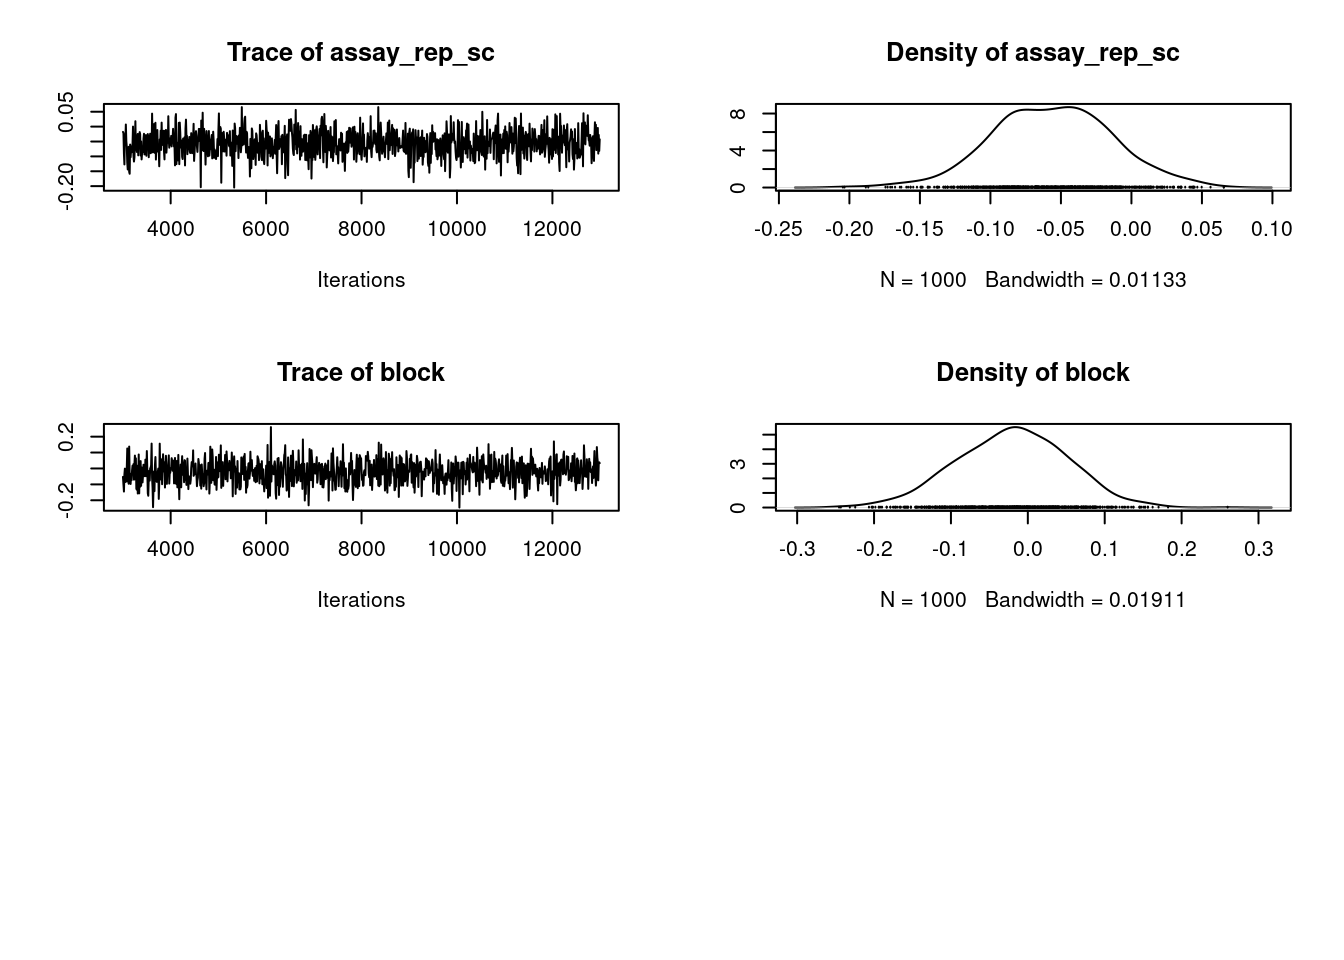
\includegraphics{02_01-glm_files/figure-pdf/unnamed-chunk-10-2.pdf}

\begin{Shaded}
\begin{Highlighting}[]
 \FunctionTok{plot}\NormalTok{(Species }\SpecialCharTok{\textasciitilde{}} \FunctionTok{log}\NormalTok{(Area), gala)}
\end{Highlighting}
\end{Shaded}

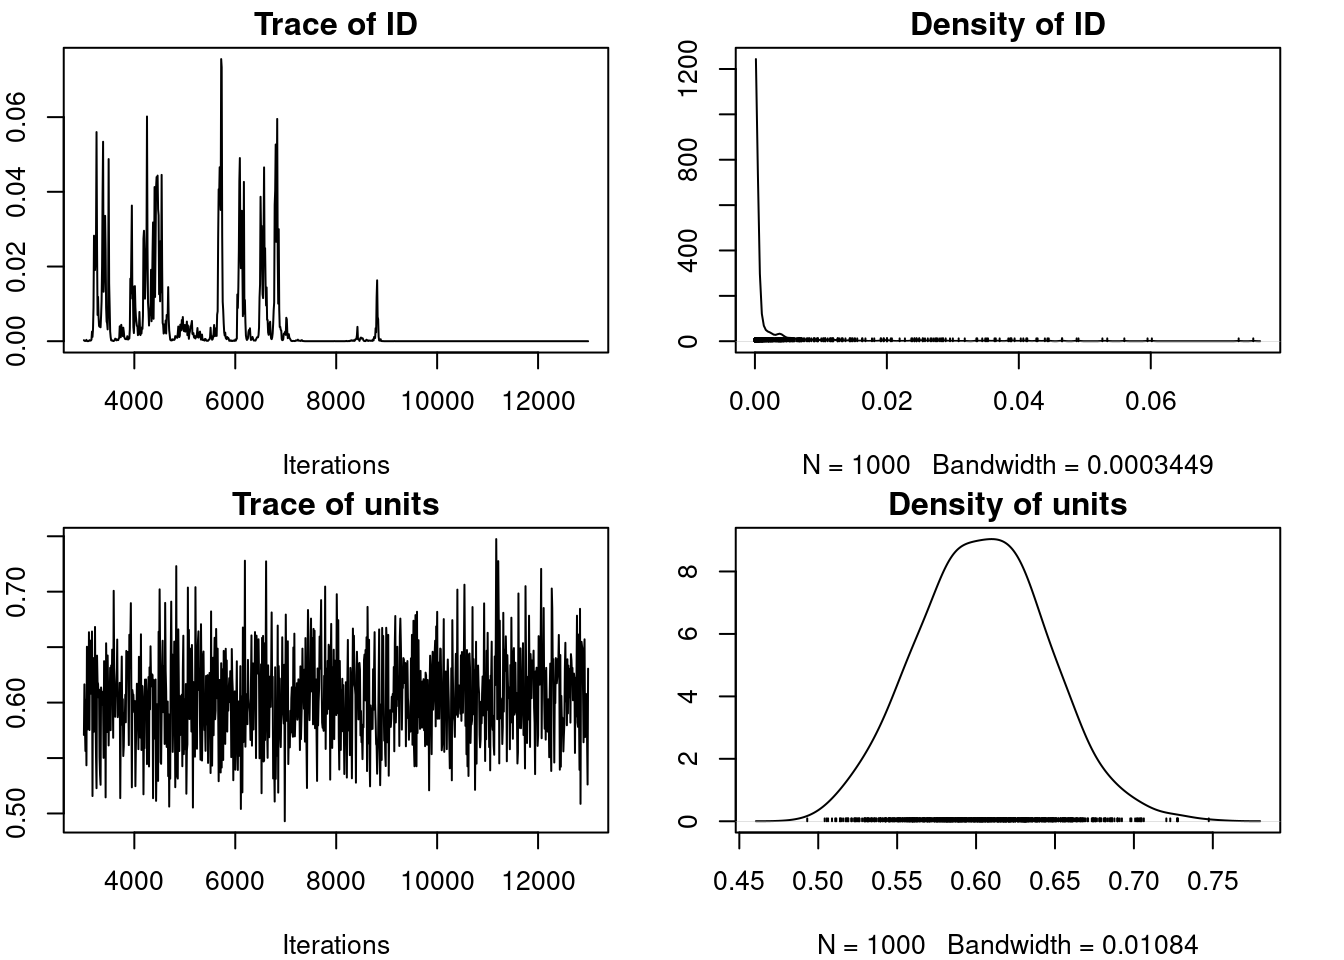
\includegraphics{02_01-glm_files/figure-pdf/unnamed-chunk-10-3.pdf}

\begin{Shaded}
\begin{Highlighting}[]
 \FunctionTok{hist}\NormalTok{(gala}\SpecialCharTok{$}\NormalTok{Species)}
\end{Highlighting}
\end{Shaded}

\includegraphics{02_01-glm_files/figure-pdf/unnamed-chunk-10-4.pdf}

\begin{Shaded}
\begin{Highlighting}[]
\NormalTok{ modpl }\OtherTok{\textless{}{-}} \FunctionTok{glm}\NormalTok{(Species }\SpecialCharTok{\textasciitilde{}}\NormalTok{ Area }\SpecialCharTok{+}\NormalTok{ Elevation }\SpecialCharTok{+}\NormalTok{ Nearest, }\AttributeTok{family=}\NormalTok{poisson, gala)}
\NormalTok{res }\OtherTok{\textless{}{-}} \FunctionTok{simulateResiduals}\NormalTok{(modpl)}
\FunctionTok{testDispersion}\NormalTok{(res)}
\end{Highlighting}
\end{Shaded}

\includegraphics{02_01-glm_files/figure-pdf/unnamed-chunk-10-5.pdf}

\begin{verbatim}

    DHARMa nonparametric dispersion test via sd of residuals fitted vs.
    simulated

data:  simulationOutput
dispersion = 110.32, p-value < 2.2e-16
alternative hypothesis: two.sided
\end{verbatim}

\begin{Shaded}
\begin{Highlighting}[]
\FunctionTok{testZeroInflation}\NormalTok{(res)}
\end{Highlighting}
\end{Shaded}

\includegraphics{02_01-glm_files/figure-pdf/unnamed-chunk-10-6.pdf}

\begin{verbatim}

    DHARMa zero-inflation test via comparison to expected zeros with
    simulation under H0 = fitted model

data:  simulationOutput
ratioObsSim = NaN, p-value = 1
alternative hypothesis: two.sided
\end{verbatim}

\begin{Shaded}
\begin{Highlighting}[]
 \FunctionTok{mean}\NormalTok{(gala}\SpecialCharTok{$}\NormalTok{Species)}
\end{Highlighting}
\end{Shaded}

\begin{verbatim}
[1] 85.23333
\end{verbatim}

\begin{Shaded}
\begin{Highlighting}[]
 \FunctionTok{var}\NormalTok{(gala}\SpecialCharTok{$}\NormalTok{Species)}
\end{Highlighting}
\end{Shaded}

\begin{verbatim}
[1] 13140.74
\end{verbatim}

\begin{Shaded}
\begin{Highlighting}[]
 \FunctionTok{hist}\NormalTok{(}\FunctionTok{rpois}\NormalTok{(}\FunctionTok{nrow}\NormalTok{(gala),}\FunctionTok{mean}\NormalTok{(gala}\SpecialCharTok{$}\NormalTok{Species)))}
\end{Highlighting}
\end{Shaded}

\includegraphics{02_01-glm_files/figure-pdf/unnamed-chunk-10-7.pdf}

\begin{Shaded}
\begin{Highlighting}[]
 \FunctionTok{plot}\NormalTok{(modpl)}
\end{Highlighting}
\end{Shaded}

\includegraphics{02_01-glm_files/figure-pdf/unnamed-chunk-10-8.pdf}

\includegraphics{02_01-glm_files/figure-pdf/unnamed-chunk-10-9.pdf}

\includegraphics{02_01-glm_files/figure-pdf/unnamed-chunk-10-10.pdf}

\begin{verbatim}
Warning in sqrt(crit * p * (1 - hh)/hh): NaNs produced

Warning in sqrt(crit * p * (1 - hh)/hh): NaNs produced
\end{verbatim}

\includegraphics{02_01-glm_files/figure-pdf/unnamed-chunk-10-11.pdf}

\bookmarksetup{startatroot}

\chapter*{References}\label{references}
\addcontentsline{toc}{chapter}{References}

\markboth{References}{References}

\backmatter

\phantomsection\label{refs}
\begin{CSLReferences}{0}{1}
\end{CSLReferences}



\printindex

\end{document}
